%%%%%%%%%%%%%%%%%%%%%%%%%%%%%%%%%%%%%%%%%%%%%%%%%%%%%%%%%%%%%%%%%%%%%%
% LaTeX Example: Project Report
%
% Source: http://www.howtotex.com
%
% Feel free to distribute this example, but please keep the referral
% to howtotex.com
% Date: March 2011 
% 
%%%%%%%%%%%%%%%%%%%%%%%%%%%%%%%%%%%%%%%%%%%%%%%%%%%%%%%%%%%%%%%%%%%%%%

% Edit the title below to update the display in My Documents
%\title{Project Report}
%
%%% Preamble
\documentclass[paper=a4, fontsize=12pt]{article}
\usepackage[T1]{fontenc}
\usepackage{fourier}
\usepackage[utf8]{inputenc}
\usepackage[french]{babel}

% English language/hyphenation
\usepackage[protrusion=true,expansion=true]{microtype}	
\usepackage{amsmath,amsfonts,amsthm} % Math packages
\usepackage[pdftex]{graphicx}	
\usepackage{url}
\usepackage[bottom=10em]{geometry}
\usepackage{float}
\usepackage{xcolor}
\usepackage{enumitem}
\renewcommand\descriptionlabel[1]{\textbf{#1 :}}
\usepackage{pdfpages}
\usepackage{rotating}

%%% Custom sectioning
%\usepackage{sectsty}
%\allsectionsfont{\normalfont\scshape}

%% Language definition package (for XML Annexe)
\usepackage{listings}
\usepackage{color}

%% Local modification of margins
\newenvironment{changemargin}[2]{\begin{list}{}{%
      \setlength{\topsep}{0pt}%
      \setlength{\leftmargin}{0pt}%
      \setlength{\rightmargin}{0pt}%
      \setlength{\listparindent}{\parindent}%
      \setlength{\itemindent}{\parindent}%
      \setlength{\parsep}{0pt plus 1pt}%
      \addtolength{\leftmargin}{#1}%
      \addtolength{\rightmargin}{#2}%
    }\item }{\end{list}}
%%

%%% Custom headers/footers (fancyhdr package)
%\usepackage{fancyhdr}
%\pagestyle{fancyplain}
%\fancyhead{}											% No page header
%\fancyfoot[L]{}											% Empty 
%\fancyfoot[C]{}											% Empty
%\fancyfoot[C]{\thepage}									% Pagenumbering
%\renewcommand{\headrulewidth}{0pt}			% Remove header underlines
%\renewcommand{\footrulewidth}{0pt}				% Remove footer underlines
%\setlength{\headheight}{13.6pt}


%%% Equation and float numbering
\numberwithin{equation}{section}		% Equationnumbering: section.eq#
\numberwithin{figure}{section}			% Figurenumbering: section.fig#
\numberwithin{table}{section}				% Tablenumbering: section.tab#

%Graphics path
%\graphicspath{./Images/}

%%% Maketitle metadata
\newcommand{\horrule}[1]{\rule{\linewidth}{#1}} 	% Horizontal rule

\title{
  %\vspace{-1in} 			
  \usefont{OT1}{bch}{b}{n}
  \horrule{1.5pt} \\[0.5cm]	
  \Huge \textbf{Rapport final} \\ [10pt]
  \Huge PFA - De la 3D vers la 2D \\ [15pt]
  \LARGE Année scolaire 2014-2015 \\ 
  \horrule{1.5pt} \\[0.5cm]
  %
}

\author{
  \huge \underline{Client} : \LARGE BLANC Carole, DESBARATS Pascal\\ [10pt] 
  \huge \underline{Encadrant} : \LARGE LOMBARDY Sylvain\\[20pt]
  \normalfont 							
  \huge \textbf{Equipe} : \Large BOHER Anaïs - CABON Yohann - CHAUVAT Magali \\[5pt]
  \Large LEVY Akané - MARCELIN Thomas \\[5pt]
  \Large MAUPEU Xavier - PHILIPPI Alexandre \\[10pt]		\normalsize
}
\date{}

%%% Begin document
\begin{document}
\maketitle

\begin{figure}[b]
  \centering
\includegraphics{logo.png}
\end{figure}

\newpage

\tableofcontents

\newpage

\begin{changemargin}{-1cm}{-1cm}

  \section{Introduction}
  \paragraph{}
        Le projet PFA a pour objectif de faire découvrir aux élèves la gestion d'un projet depuis la création du cahier des charges jusqu'à l'implémentation en ayant à faire à des clients réels. C'est le premier projet du cursus se réalisant avec un groupe de taille conséquente (en moyenne 7 personnes) et dans lequel les élèves établissent en échangeant avec le client les spécifications. Celui-ci se déroule sur les deux semestres, et se décompose en deux phases. Une première phase durant le premier semestre pour établir les besoins, et les présenter de manière formelle dans le cahier des charges. Puis la deuxième au cours du second semestre pour concrétiser ces besoins en réalisant ce qui est spécifié.

\paragraph{}      
        Le projet PFA effectué : De la 3D à la 2D, est un projet d'imagerie numérique. L'objectif est de réaliser une scène 3D constituait de un ou plusieurs modèles 3D pour ensuite générer des images en deux dimensions de celle-ci permettant de recréer une illusion de trois dimensions en se basant sur des principes connus. Les algorithmes étudiés au cours de ce projet permettent de générer des anaglyphes, autostéréogrammes et folioscopes qui seront présentés plus en détails dans la suite du rapport.
        
\paragraph{}
        Pour commencer le domaine de la synthèse d'image et les différents rendus à implémenter dans le logiciel seront présentés, puis brièvement les besoins visés lors de la phase d'écriture du cahier des charges avant de parler finalement de l'implémentation du projet.

  \newpage

  \section{Présentation du projet}
  Cette partie présente le domaine de la synthèse d'image ainsi que le sujet du projet. Nous y présenterons également les besoins du futur logiciel qui ont été déterminés à partir de ces recherches.
  \subsection{Domaine}
  \paragraph{}
	Ce projet s’inscrit dans le domaine de la synthèse d’images et de la visualisation de modèles en trois dimensions. Depuis le quinzième siècle, grâce à la peinture, la perspective apparaît sur des supports en deux dimensions. Aux XIXème et XXème siècles, l’utilisation de stéréoscopes, tel que le stéréoscope de Holmes, permettait la visualisation de relief à partir de deux images planes et d’un dispositif optique. Dans la deuxième moitié du XXème siècle, l’utilisation du numérique permet de modifier les images et d’obtenir une meilleure visualisation de la profondeur sur des supports en deux dimensions. 

\paragraph{}	
	On peut ainsi créer des anaglyphes, des autostéréogrammes ou des flipbooks, qui sur papier ou sur écran permettent d’apercevoir la profondeur d’une scène grâce à des techniques adaptées. Ces différents rendus seront présentés plus tard dans ce cahier des charges. De nos jours, il existe également des logiciels, tels que Meshlab et Blender qui sont gratuits, open source et permettent d’ores et déjà la visualisation en trois dimensions sur un écran. L’utilisateur peut tourner autour d’un objet et le voir sous tous ses angles grâce à un ensemble de projections successives autour de l’objet.

\paragraph{}
	On appelle synthèse d’image l'ensemble des techniques qui permettent de visualiser des objets en trois dimensions en perspective sur un écran d'ordinateur, en tenant compte de lumières et de textures appliquées à l'objet. Il existe un grand nombre de techniques et les résultats obtenus peuvent eux aussi varier (perspective isométrique, perspective conique...). Nous nous préoccupons par la suite de la perspective conique, dite aussi vue naturelle. 

\paragraph{}
	Bien souvent, la synthèse d'image utilise le principe de scène. Il s'agit d'un espace à trois dimensions dans lequel des objets peuvent être placés. Ces derniers sont décrits par un ensemble de points placés dans l'espace.

\paragraph{}
	Pour pouvoir observer la scène et les objets, il est nécessaire de demander à l'ordinateur de les modéliser, c'est-à-dire d'afficher un rendu qui correspondrait à une vision de cette scène si elle était réelle. Pour cela, la machine simule le point de vue de l'utilisateur à l'aide d'une « caméra ». A partir de cette scène en trois dimensions, la caméra peut réaliser des projections ou photographies permettant de créer des anaglyphes, autostéréogrammes ou flipbooks. Plusieurs méthodes de projection existent, mais seule celle par matrice de projection sera utilisée.

\paragraph{}
	Ces matrices sont décrites à l’aide de coordonnées homogènes. Celles-ci ont été introduites afin que l’ensemble des transformations de type rotation, translation et homothétie puissent être écrites sous forme de matrice. Ainsi, le produit des matrices de transformation peut être calculé en amont pour pouvoir appliquer la matrice de la transformation résultante à l’ensemble des points de l’objet sans avoir à recalculer le produit pour chaque point.

\paragraph{}
	Pour pouvoir visualiser un modèle 3D il faut prendre en considération la lumière et sa réflexion sur l’objet. Si une sphère rouge était représentée dans un espace avec uniquement une lumière ambiante, il n’en ressortirait qu’un disque rouge, sans relief. En effet, la lumière ambiante atteint l’objet de la même façon en tout point. On ne peut donc pas savoir depuis un plan fixe s’il s’agit d’un objet en deux ou en trois dimensions. Si maintenant une lumière est ajoutée dans l’espace où est situé l’objet, celle-ci ne va pas atteindre tous les points de l’objet de la même façon. Elle sera plus faible sur un point plus éloignée, voire inexistante sur un point caché. En tenant compte de cette lumière, on peut obtenir une image comme présentée sur la figure \ref{fig:sphère}.

\begin{figure}[h]
	\centering
	
\includegraphics[scale=0.3]{boule.png}
	\caption{\label{fig:sphère} Application d’une lumière diffuse à une sphère rouge \protect \footnotemark }
\end{figure}
\footnotetext{http://linut.free.fr/omgspl0kuberwebloglolz0r/?2010/02/01/93-raytracer-que-la-lumiere-soit}

\paragraph{}
	Pour la création d’un anaglyphe, deux images espacées par une petite distance (qui correspond à la distance entre les deux yeux par exemple) sont générées. La composante rouge de l’une de ces images et la composante bleue de l’autre sont gardées et ensuite superposées dans une même image. Cette image est ensuite transformée en une image Rouge-Cyan, qui peut être visualisée à l’aide de lunettes Rouge-Bleue : l’image apparaît en trois dimensions.

\paragraph{}
	Pour la création d’un autostéréogramme, une image permettant d'observer un objet en relief par vision parallèle est générée. Cette image est obtenue à partir d'une texture de base ou de points aléatoires pour l'image de fond.

\paragraph{}
	Pour la création d’un flipbook, plusieurs images sont prises à intervalles réguliers par une caméra suivant un trajet prédéterminé dans ou autour de la scène. Le flipbook est visualisable en faisant rapidement défiler ces images tout en respectant l’ordre des prises de vue. Ce flipbook peut être transformé en GIF pour obtenir une visualisation animée des images.

  \subsection{Sujet du projet}
  présentation du sujet
reprendre présentation du cahier des charges
améliorer avec une vision plus poussée du projet

\paragraph{}
	Le projet concerne la réalisation d’un logiciel permettant d’obtenir des projections en deux dimensions, des anaglyphes, des autostéréogrammes ou encore des flipbooks à partir de scènes virtuelles en trois dimensions. 

\paragraph{}
	L’objectif premier est de permettre la visualisation, sur un support en deux dimensions tel qu’un écran d’ordinateur ou une feuille de papier, d’un espace en trois dimensions. A partir de la visualisation d’objets 3D dans une scène il faudra donc réaliser des photographies qui une fois traitées donneront lieu à des anaglyphes, autostéréogrammes ou des animations type flipbook.
	
\paragraph{}
	Afin d’atteindre cet objectif, un logiciel s’appuyant sur le moteur 3D OpenGL devra être réalisé. Il permettra la création d’une scène où s’inséreront des objets dont la position, la taille et l’orientation seront paramétrables. Une caméra permettra de se déplacer dans la scène, de s’en rapprocher ou s’en éloigner.

\paragraph{}
	Une fois la scène mise en place, il faudra pouvoir prendre des photographies de celle-ci sous différents angles afin d’obtenir, après application d’algorithmes de traitement d’images :

\begin{itemize}
	\item
		des anaglyphes rouge-cyan, qui permettront une visualisation en trois dimensions grâce à des lunettes adaptées ;
	\item
		des stéréogrammes, qui sont des images dissimulant un contenu qui apparaît quand on fixe le dessin de façon spécifique ;
	\item
		des flipbooks ou images animées, correspondant à une succession d’images suivant une trajectoire qui permettent en les faisant défiler de donner une impression de mouvement.
\end{itemize}

  \subsection{Présentation des rendus souhaités}
  Cette partie présente les trois rendus qui ont été implémentés pour le logiciel : l'anaglyphe, l'autostéréogramme et le folioscope.
  \subsection{Les flipbooks}

\paragraph{}
	Le principe d’un flipbook, ou folioscope en français, est de créer une suite d’images successives d’une scène par rapport à une trajectoire. Il suffira ensuite de mettre toutes ces images dans l’ordre les unes derrière les autres, et de les faire défiler rapidement pour avoir l’impression d’un rendu en relief et en mouvement. C’est également le principe des fichiers d’extension .GIF, qui font défiler une liste d’images.

        \footnotetext{OpenGL perspective projection : \url{http://www.3dcpptutorials.sk/index.php?id=2}}
        
\paragraph{}
	La création d’un flipbook est possible en créant une animation à l’aide d’un logiciel de manipulation d’objets 3D et en ne capturant que certaines images, par exemple avec Blender. Ainsi l’impression de ces images successives permet de réaliser un flipbook (cf. figure \ref{fig:flipbook}). En combinant par exemple avec le logiciel Gimp (outil d’édition et de retouche d’image) l’animation peut être obtenue en GIF. 

\begin{figure}[h!]
		\centering
		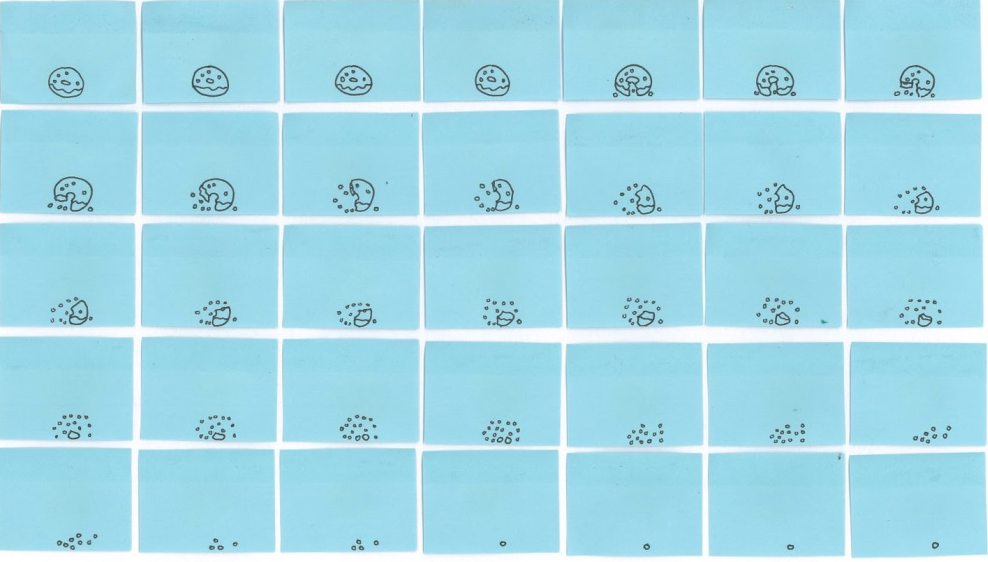
\includegraphics[scale=0.7]{flipbook.png}
		\caption{\label{fig:flipbook} Story-board d’un flipbook \protect \footnotemark }
\end{figure}
\footnotetext{\url{http://tracieliu.blogspot.fr/2010/08/flipbook-storyboard.html}}

\subsection{Les autostéréogrammes}	

\paragraph{}
	Un autostéréogramme est une image qui cache une visualisation en trois dimensions d’un objet. Cette image est construite de sorte qu'à chaque point de l'objet en trois dimensions soient associés deux points de l'image. L'utilisateur doit observer chaque point d'un couple de points avec un seul œil, ce qui donne l'illusion au cerveau d'observer deux images différentes avec les deux yeux et donc l'incite à traiter cette information comme l'observation d'un objet en trois dimensions, comme illustré par la figure \ref{fig:ppe_autostereogramme}.

\paragraph{}
	La visualisation en trois dimensions peut être difficile à obtenir, et demande une réelle gymnastique oculaire. Il faut pouvoir fixer le regard en avant ou en arrière de l’image, pour réussir à y voir l’objet caché. La plupart des autostéréogrammes sont observables en vision parallèle, c'est-à-dire qu'il faut faire le point au-delà de l'image pour pouvoir observer l'objet.

\begin{figure}[h]
  \centering
  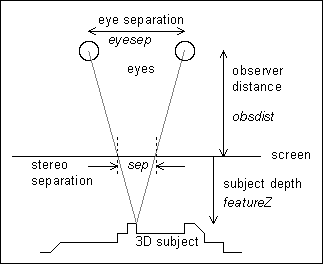
\includegraphics[scale=0.5]{./ppe_autostereogramme.png}
  \caption{Visualisation d’un autostéréogramme en vision parallèle \protect \footnotemark }
  \label{fig:ppe_autostereogramme}
\end{figure}

\footnotetext{\url{http://www.techmind.org/stereo/geometry.gif}}

\paragraph{}
	Pour générer un autostéréogramme, il faut utiliser une carte des profondeurs, ou carte de disparité, de l’objet à dissimuler. Cette carte s’obtient grâce à deux visions d’une même scène prises à deux endroits différents, et permet de mettre en avant les informations sur la profondeur de l’objet. Par exemple, la carte des profondeurs de la figure \ref{fig:carteProfondeur} a permis d’obtenir l’autostéréogramme de la figure \ref{fig:autostereogramme}.

\begin{figure}[h]
		\centering
		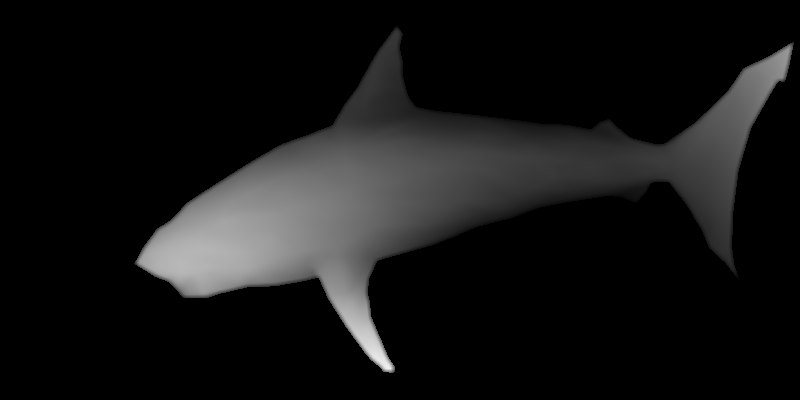
\includegraphics[scale=0.2]{carteProfondeur.png}
		\caption{\label{fig:carteProfondeur} Carte des profondeurs \protect \footnotemark }
\end{figure}
\footnotetext{\url{http://en.wikipedia.org/wiki/Autostereogram}}

\begin{figure}[h]
		\centering
		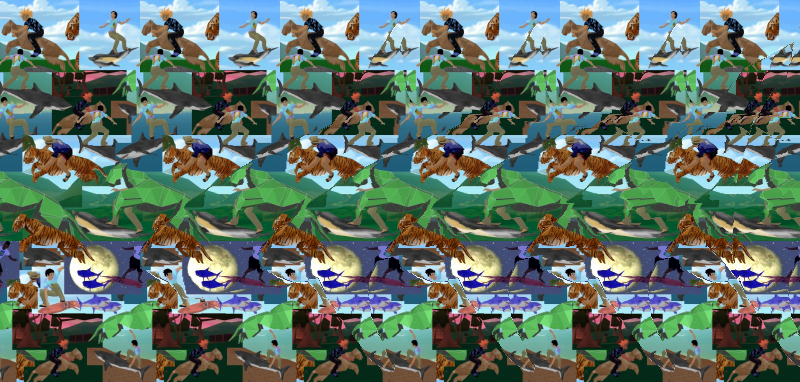
\includegraphics[scale=0.4]{autostereog.png}
		\caption{\label{fig:autostereogramme} Autostéréogramme obtenu \protect \footnotemark }
\end{figure}

\paragraph{}
Il existe des algorithmes de génération d’autostéréogrammes très simples , comme celui proposé par Gary Beene \cite{garybeene}. Cependant un algorithme aussi peu optimisé produit des autostéréogrammes défecteux, comportant par exemple des échos (répétition d'une partie de l'objet 3D) ou des artefacts (défaut de l'objet 3D observé).

\paragraph{}
Des algorithmes plus poussés ont été développés, comme celui présenté par Harold W. Thimbleby, Stuart Inglis et Ian H. Witten \cite{stereogram}, et celui proposé par W. A. Steer \cite{wasteer}, associés à une réalisation en C. Ils permettent la génération d’autostéréogrammes SIRDS (Single Image Random Dots Stereogram) à partir d’une image 2D. Ces articles présentent également des méthodes de correction de problèmes tels que l'écho ou la gestion des faces cachées (faces de l'objet tridimensionnel visibles par un seul œil). W. A. Steer propose de plus une méthode de génération d'autostéréogrammes utilisant un motif bitmap comme image de base plutôt qu'un nuage de points aléatoires, ce qui pallie à certaines limites des SIRDS comme le manque de détails et la grossièreté des surfaces courbes.
\footnotetext{\url{http://en.wikipedia.org/wiki/Autostereogram}}


\subsection{Les anaglyphes}

\paragraph{}
	Un anaglyphe est une image sur laquelle on superpose deux vues, si possible différentes, d’une scène. La meilleure distance entre ces deux visions est la même que celle entre les deux yeux, afin que le cerveau puisse recréer la même vision en trois dimensions que dans la réalité.
	
\paragraph{}
	Les anaglyphes les plus fréquents sont les anaglyphes dits rouge-cyan. Ils se nomment ainsi car ils sont constitués d’une image sur laquelle on passe un filtre magenta, et une autre avec un filtre cyan (cf. figure \ref{fig:anaglyph}). Pour pouvoir visualiser le relief sur une telle image, on utilise une paire de lunettes rouge-cyan, dont chaque verre est un filtre pour l’une des deux couleurs de l’image. Le plus souvent, le filtre magenta est placé sur l’œil gauche, le cyan sur l’œil droit. En regardant l’image, l’œil gauche ne verra alors que la composante cyan, et inversement pour l’œil droit. Les deux images ayant un léger décalage, le cerveau va percevoir l’image comme si elle était en trois dimensions. Les anaglyphes rouge-cyan sont principalement intéressants sur des images en noir et blanc. En effet, quand il s’agit d’images en couleur, celles-ci sont souvent détériorées par l’usage des filtres, car les couleurs possèdent généralement de plusieurs composantes. A l’inverse, quand l’image est en nuances de gris, l’image n’est pas modifiée, juste mise en relief. Plusieurs types d'algorithmes existent pour créer des anaglyphes depuis des paires d'images. Ils se différencient par la qualité de l'anaglyphe en sortie en diminuant le nombre d'artefacts \cite{steteroAnaglyph} ou en améliorant le rendu pour l'impression \cite{printAnaglyph} par exemple.

\begin{figure}[h]
		\centering
		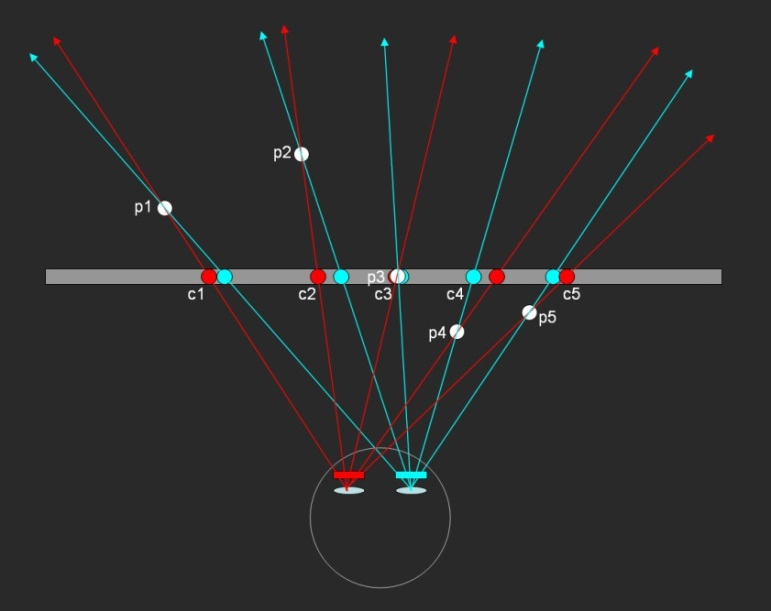
\includegraphics[scale=0.8]{anaglyph.png}
		\caption{\label{fig:anaglyph} Le décalage de la partie rouge et cyan permet à l’œil de percevoir l’image non plus dans un plan XY mais dans l’espace \protect \footnotemark }
\end{figure}
\footnotetext{\url{http://www.david-romeuf.fr/3D/Anaglyphes/TCAnaglypheLSDubois/TransformationCouleursPourAnaglyphe.html}}

\paragraph{}
	Le paragraphe précédent concernent la création d’un anaglyphe depuis deux prises de vue d’une même scène avec un léger décalage. Mais il est également possible de le faire à partir d’une image en deux dimensions grâce à l’algorithme de Dubois \cite{algoDubois}, qui définit une vision matricielle de l’anaglyphe (cf. figure \ref{fig:algoDubois}). Dès lors, une matrice de transformation est introduite, qui permet de passer du taux RGB d’un pixel de l’image originale,  aux deux taux RGB des anaglyphes gauche/droite. Les coefficients de cette matrice sont calculés pour satisfaire une bonne restitution de l’image originale, tout en supprimant les rivalités colorées induites par des lunettes bicolores. Ainsi, pour visualiser une image rouge pure, il faudra changer le taux RGB de ce pixel pour que les deux yeux puissent le voir après les filtres. Sinon l’information ne circulera que dans un œil, et l’on perdra la vision stéréoscopique, et donc la notion de profondeur. 
	
\begin{figure}[H]
		\centering
		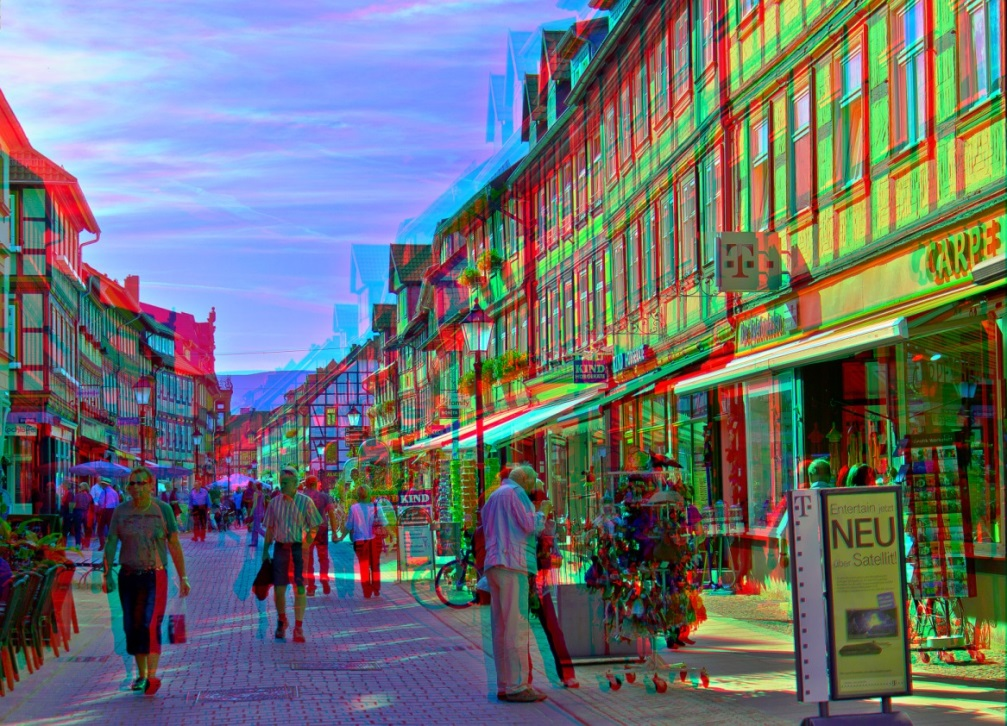
\includegraphics[scale=0.9]{algoDubois.png}
		\caption{\label{fig:algoDubois} Rendu final d’une image par l’algorithme de Dubois \protect \footnotemark }
\end{figure}
\footnotetext{\url{http://zour.deviantart.com/art/Wernigerode-Boulevard-Dubois-Anaglyph-HDR-3D-276542278}}
	
	

  \subsection{Résumé du cahier des charges}
  retour sur la rédaction du cahier des charges
aide du client (cours du début pour ce qu'il attendait comme contenu)
suivi hebdomadaire pour contrôler l'avancée et nous orienter pour un cahier des charges comme il l'attendait
méthode de travail, recherches, prototypes

\paragraph{}
        Dans le cadre du projet PFA, la première partie consistait à rédiger un cahier des charges fonctionnel pour définir l'ensemble des besoins du futur logiciel.

\paragraph{}
        Lors de notre premier rendez-vous, notre client a d'ores et déjà défini le format qu'il souhaitait pour le cahier des charges, et le contenu qui était essentiel pour lui. Il fallait ainsi présenter le domaine d'études et les connaissances actuelles sur des algorithmes de création d'anaglyphes, d'autostéréogrammes ou de folioscopes. Ensuite, le sujet était à redéfinir précisément, puis les besoins fonctionnels et non fonctionnels demandés par les clients pour ce logiciel, ainsi que les contraintes engendrées par ceux-ci. Enfin, il fallait présenter des prototypes permettant de répondre aux différents besoins ennoncés, quelques interfaces graphiques pour simuler l'utilisation du logiciel, et surtout réfléchir à l'architecture future du projet.

\paragraph{}
        La rédaction des parties Domaine et Etat de l'existant aura demandé de nombreuses recherches, notamment pour trouver des articles présentant des algorithmes de création d'anaglyphes et d'autostéréogrammes. 
L'étude du domaine aura permis de se familiariser avec le vocabulaire de la synthèse d'image et avec les différents rendus souhaités par nos clients. Des notions telles que la scène, la caméra, ainsi que la compréhension du fonctionnement des anaglyphes et des autostéréogrammes, auront ainsi permis une meilleure immersion dans notre projet.
Les algorithmes relatifs aux anaglyphes concernent principalement le traitement des couleurs pour qu'aucun artefact n'apparaisse au moment de la visualisation finale. Pour les autostéréogrammes, le traitement d'une carte des profondeurs permet d'obtenir une image qui, lorsque l'on sait l'observer, fait apparaître un relief. Enfin, il n'existe pas d'algorithme particulier pour la génération de folioscopes. Seule une série de prises de vue d'une scène avec des angles d'observation proches peuvent permettre, si elles sont visualisées les unes à la suite des autres et suffisamment rapidement, de pouvoir imaginer un mouvement, et ainsi un relief.

\paragraph{}
        Les besoins fonctionnels et non fonctionnels d'un projet doivent impérativement être ciblés durant la phase de cahier des charges, car c'est grâce à eux que le contrat passé entre les clients et l'équipe de programmeurs pourra être exhaustif et protéger les deux parties contre d'éventuelles envies de modification au cours de la phase de réalisation. 
Pour un tel logiciel, les besoins fonctionnels s'apparentent bien souvent à de futures fonctionnalités du logiciel, tel que la création d'une scène, sa manipulation, et les prises de vue pour obtenir les rendus demandés dans le sujet. 
Toutefois, les besoins non fonctionnels, même s'ils peuvent être clairement énoncés par le client, sont bien souvent implicites et doivent être déterminés en fonction du discours tenu. Pour un logiciel de synthèse d'images, la fluidité d'affichage est bien souvent un besoin essentiel, car l'utilisateur s'attend à une certaine rapidité du logiciel lors de la manipulation de la scène et de la génération de rendus. Mais d'autres besoins, à savoir la portabilité du logiciel et sa maintenabilité, ont également été exprimés par les clients et ont été considérés comme essentiels pour ce projet. En effet, l'utilisaton de ce logiciel, au moins sous les systèmes d'exploitation Linux et Windows, était importante pour pouvoir travailler sur différentes machines dans leur travail. De plus, un tel logiciel pouvait être amené à être amélioré ou réutilisé en partie dans de futurs projets, et c'est pourquoi il devait être facilement maintenable.
Ces besoins ont apportés des contraintes quand à la réalisation du logiciel, par exemples sur les langages et les bibliothèques utilisées. Les choix ainsi effectués pour permettre de tenir ces contraintes seront détaillées par la suite.

\paragraph{}
Pour s'assurer de la faisabilité des besoins fonctionnels et non fonctionnels du projet, deux prototypes ont été mis en place : un prototype de fichier XML pour réfléchir au format de sauvegarde et de chargement de la scène, et un prototype de scène en trois dimensions pour tester les fonctionnalités possibles avec le langage C++ et les bibliothèques que nous souhaitions utiliser : Qt et OpenGL pour Qt. Ce prototype aura également permis de s'assurer de la portabilité de ces bibliothèques, ainsi que de la fluidité potentielle du futur logiciel.
Le prototype XML aura permis de réfléchir aux informations importantes à stocker pour pouvoir recréer une scène à l'identique. Tout d'abord, les informations relatives aux objets doivent être stockées, telles que leur nom et leur fichier d'origine, mais également leur position, leur orientation et leur échelle. Les informations relatives à la caméra sont également essentielles pour retrouver l'angle d'observation de la scène, et les informations à stocker sont sa position, son orientation, ou encore son angle de vue. Le prototype d'origine du fichier XML est donné dans la partie Annexe du Cahier des Charges, lui-même présent en Annexe de ce rapport. Un exemple de fichier XML obtenu à partir de ce prototype est également donné en Annexe.
Le prototype logiciel réalisé en C++ a permis de mettre en place une première version de scène contenant un objet obtenu grâce à une première version de parseur de fichiers d'extension PLY. La manipulation de cette scène a permis de tester quelques valeurs de fluidité pour pouvoir se rendre compter des capacités d'affichage des bibliothèques utilisées, qui semblaient satisfaire nos attentes. De plus, le test du prototype sur des machines Windows et Linux ont montré la portabilité des bibliothèques, même si les versions de shaders utilisées auront posé problème par la suite comme il est détaillé dans la partie suivante de ce rapport. Un exemple d'affichage du prototype initial est donné dans la [FIGURE N°], et des exemples de l'affichage final seront donnés plus tard dans ce rapport.

\paragraph{}
Pour satisfaire le besoin d'extensibilité de notre projet, nous avons mis en place une architecture modulaire pour permettre à notre logiciel d'être modifié de façon simple. L'architecture principale est donné dans la [FIGURE].

//figure

Les besoins en modularité de notre projet se reflète particulièrement dans le paquetage Création de l'architecture, qui permet la création des différents rendus que le logiciel permet d'obtenir. L'architecture de ce paquetage est donné dans la [FIGURE N°]

//figure

L'extensibilité de cette architecture se traduit principalement par l'utilisation d'interfaces à différents niveaux. Tout d'abord, le Creator, point d'entrée du paquetage, a pour attribut une première interface Creation qui peut devenir n'importe lequel des rendus souhaité par l'utilisateur. Il peut donc aussi bien devenir un anaglyphe qu'un autostéréogramme. Toutefois, pour permettre l'utilisation de divers algorithmes pour réaliser un même rendu, les classes des rendus sont également des interfaces dont héritent les classes réellement instanciables qui correspondent chacune à un algorithme. On aura donc par exemple AnaglyphAlgorithm1 ou encore DepthMapAlgorithm2.

  \newpage


  \section{Déroulement de la réalisation technique}
  Nous présenterons dans cette partie les choix faits pour la réalisation du logiciel concernant le langage, les bibliothèques et les algorithmes des rendus, et nous détaillerons les étapes de la réalisation.

  Une notice d'installation et une notice d'utilisation de notre logiciel Project3Donuts sont fournies en Annexe de ce rapport, ainsi que les conventions de codage qui ont été utilisées.

  \subsection{Choix de programmation}
  \paragraph{}
        Pour la réalisation du projet, nos clients nous proposaient des langages comme le C, le C++ ou encore le Python. Le C++ nous est apparu comme le choix le plus judicieux pour notre logiciel. En effet nous voulions un langage orienté objet, pour avoir du code lisible et une architecture claire. L'utilisation du C++11 nous permet d'utiliser entre autres les \texttt{std::unique\_ptr} pour limiter les risques de fuite de mémoire ou les lambda expressions pour garder en mémoire les actions de l'utilisateur.

    Comme nous l'avons exprimé plus haut, l'un des besoins non fonctionnels primordiaux de notre projet est la maintenabilité du code. Pour celà, il nous fallait choisir des outils et des bibliothèques qui étaient destinées à perdurer le plus longtemps possible.
    
    L'utilisation de Qt et d'OpenGL est assez répandue pour des logiciels de visualisation et de manipulation en trois dimensions. De plus Qt est très complet et propose un vaste choix de modules qui permettent de traiter un ensemble très variable de tâches (par exemple l'analyse de fichiers XML ou la gestion d'évènement). Comme ces bibliothèques sont portables, elles convenaient parfaitement à l'implémentation que nous souhaitions réaliser.
    
    La version 5 de Qt est la plus récente actuellement, mais malgré sa jeunesse elle est devenue au fil des modifications suffisament stable pour pouvoir être utilisée sans problème, et elle dispose d'une communauté Internet active prête à aider en cas de difficultés de code. De plus, cette bibliothèque utilise la version ES 2.0 de OpenGL, qui est une version non seulement qui utilise des shaders, mais également qui peut être utilisée pour de la programmation d'applications mobile par exemple. C'est donc pour ces raisons que nous avons choisi d'utiliser ces bibliothèques et ces versions.

    Pour la compilation du projet et des bibliothèques, nous avons choisi d'utiliser CMake, qui est répandu et portable. Nous aurions pu choisir également QMake, mais celui-ci dépendant trop fortement de QtCreator, nous avons préféré ne pas l'utiliser.

  \subsection{Rendu 2D}
  \paragraph{}
L'ensemble des rendus est réalisé avec OpenGL et des shaders écrits en GLSL. Lorsque un objet est chargé dans la scène, le chargeur d'objet remplit des tableaux tels que la position des sommets, les couleurs et les normales associées aux sommets, et les indices associés aux sommets de chaque faces.\\
Le problème est que certains fichiers d'objet, notamment les fichiers avec le format .ply, ne possèdent pas d'information sur les couleurs et les normales des sommets. Or ces informations sont indispensables pour avoir un beau rendu 2D. Ainsi si ces informations sont manquantes, la couleur de l'objet est mise à grise par défaut et les normales sont recalculées à partir de l'orientation des faces.

\paragraph{}
Toutes les informations sur l'objet sont placées dans un VAO (Vertex Array Object) et transmises une seule fois à la carte graphique lors de l'initialisation. Ensuite ce VAO est traité pour chaque rendu par des shaders.\\
Cette technique présente l'avantage d'envoyer le VAO une seule fois à la carte graphique alors qu'avec la méthode du rendu sans shaders, les données de l'objet sont envoyées à chaque rendu, ce qui le ralentit considérablement.

\paragraph{}
Sans shaders les rendus n'étaient pas esthétiques, comme le montre la figure \ref{fig:screenRenduSansShader.png}. L'ombrage n'était pas doux et la frontière entre chaque face était clairement visible.\\
Les shaders ont pu remédier à cela grâce à la technique du \textit{per-pixel lighting} : l'ombrage n'est plus calculé face par face mais pixel par pixel, ce qui offre une plus grande précision et ce qui permet de lisser l'ombre.\\

\begin{figure}[h!]
	\centering
	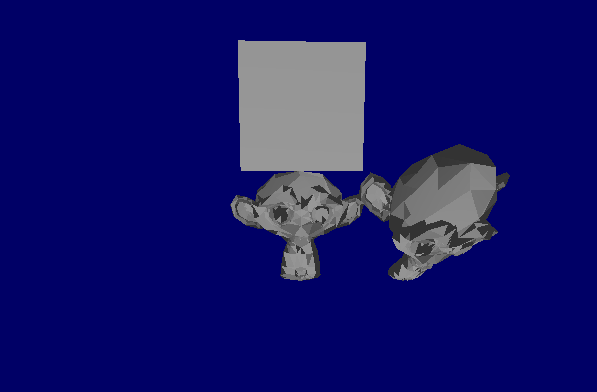
\includegraphics[scale=0.47]{images/rendu_sans_shader.png}
        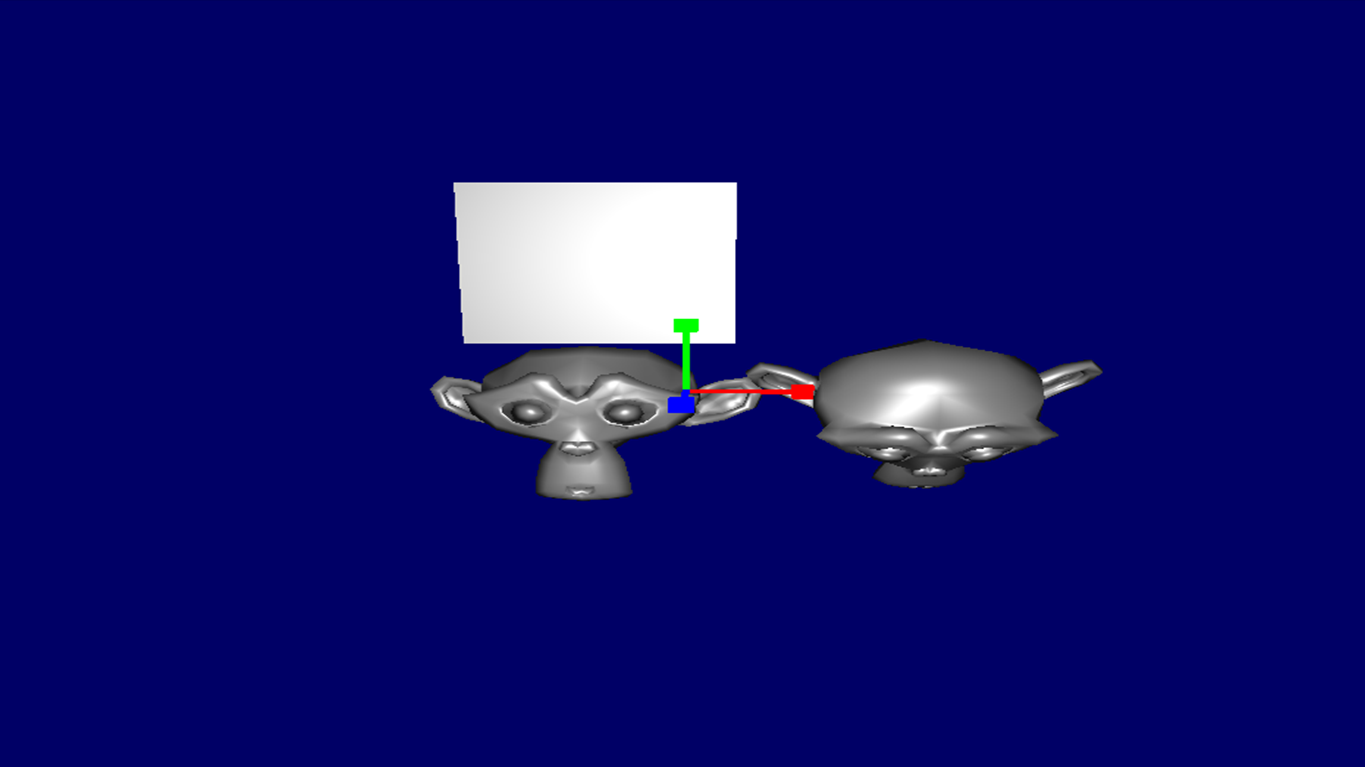
\includegraphics[scale=0.3]{images/singe_shaders.png}
	\caption{\label{fig:screenRenduSansShader.png} Comparaison de rendu avec et sans shaders \protect}
\end{figure}

\paragraph{}
Pour améliorer le rendu, il a été choisi de rajouter une spécularité à l'aide du shader. Cet effet permet de simuler les réflections de lumière sur l'objet, comme le montre la figure \ref{fig:screenSpecular.png}.


\begin{figure}[h!]
	\centering
	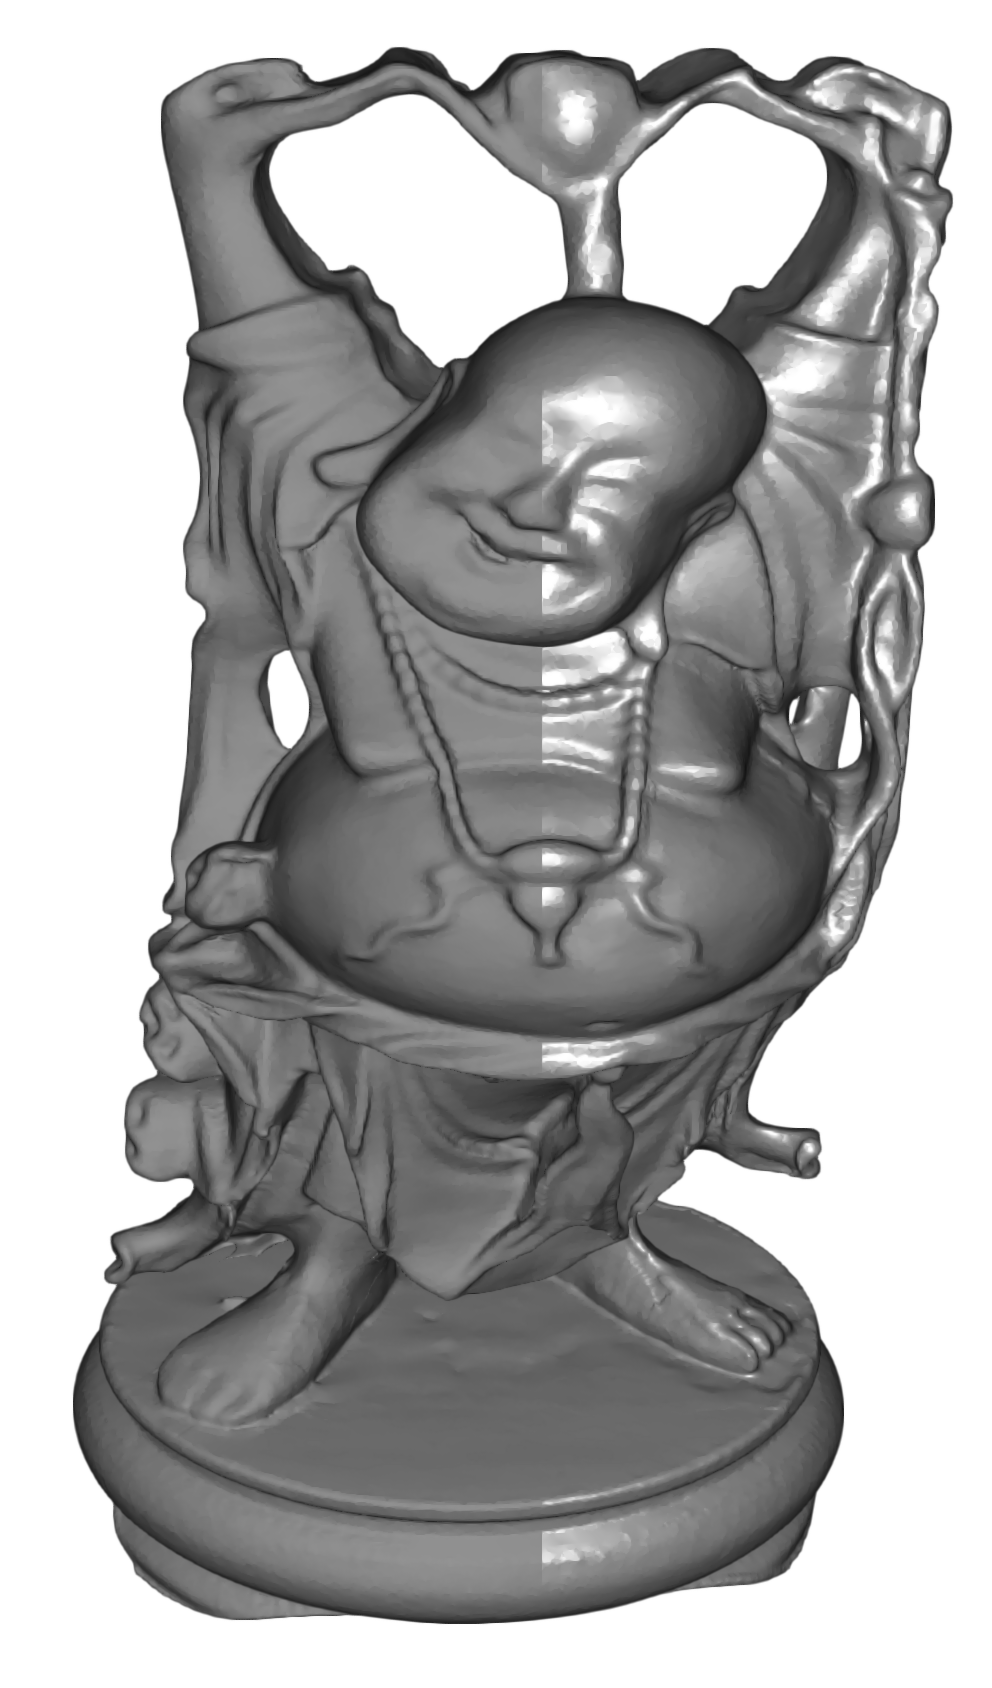
\includegraphics[scale=0.23]{images/rendu_specular.png}
	\caption{\label{fig:screenSpecular.png} Rendu avec l'ombrage de base à gauche et avec la spécularité à droite. \protect}
\end{figure}

  \subsection{Choix des algorithmes d'anaglyphes}
  Cette partie présentera les différents algorithmes qui ont été choisis pour générer des anaglyphes dans le logiciel.

\subsubsection{La génération des anaglyphes et ses défauts}
	L'anaglyphe est une image issue d'un traitement particulier sur deux prises de vue stéréoscopiques et qui nécessite des lunettes spécifiques composées d'un filtre rouge (ou magenta ou jaune) pour un \oe il et cyan (respectivement vert ou bleu) pour l'autre. 
	
	La génération des anaglyphes passe par trois étapes essentiellement. Tous d'abord, une prise de vue stéréoscopique d'une scène 3D avec les deux points de vue éloignés d'une distance proche de celle entre les yeux, de manière à obtenir une vue pour chaque \oe il, est nécessaire. Ensuite, un traitement est opéré sur ces deux images, avec au minimum l'application de deux filtres rouge et cyan (ou deux autres couleurs correspondants à celles des lunettes). Finalement, les deux images résultantes sont superposées pour n'obtenir qu'une seule image qui pourra être visionnée à travers les lunettes avec une impression de trois dimensions.
	
	Les algorithmes de génération des anaglyphes proposent des traitements d'image différents (deuxième étape) ayant pour but d'améliorer la qualité des anaglyphes. Un critère important pour juger de la qualité des anaglyphes est l'absence d'artefacts. Il s'agit de perceptions d'un phénomène de diaphonie qui est le résultat d'une mauvaise séparation des deux vues (un \oe il perçoit un détail de la vue destiné à l'autre \oe il), et dégradent l'impression de trois dimensions. %parler des rivalités binoculaire..? 

	Cependant, aucun algorithme ne peut être parfait, comme il est expliqué dans l'article d' Andrew J. Woods et Chris R. Harris \cite{anaglypheDefaut}  : la qualité de l'anaglyphe dépend de l'image, des lunettes employées et du support affichant l'image (l'article traite principalement les écrans mais il en va de même pour des anaglyphes imprimés avec le choix du papier). Hormis les lunettes, les deux autres facteurs ont toujours été problématiques pour le traitement d'image en général.  
	
	Pour obtenir des algorithmes très performants, il faudrait prendre en compte tous ces facteurs et adapter au cas par cas. En effet, étant donné que les différentes caractéristiques (luminosité, résolution,) varient pour chaque écran, obtenir une même couleur sur deux écrans distincts (produits par des entreprises différentes) suppose un calibrage au préalable ou l'utilisation d'une palette de couleur limitée. Ainsi, les techniques employés dans le domaine de recherche de la génération des anaglyphes restent très souvent basées sur des connaissances empiriques.
		
	Nous avons choisi d'implémenter deux méthodes qui permettent d'obtenir des images de qualité différentes, pour que l'utilisateur puisse choisir pour chaque donnée entrée l'algortihme qui rendra l'anaglyphe de meilleure qualité. %phrase a reprendre...
	  
\subsubsection{La méthode Photoshop}
	Le premier algorithme implémenté est le plus basique : c'est la méthode dite Photoshop qui se contente d'appliquer les deux filtres de couleur sans réaliser d'autres traitements d'image. Cette méthode est décrite dans l'article rédigé par W. Alkhadour, S. Ipson, J. Zraqou, R. Qahwaji et J. Haigh \cite{steteroAnaglyph}. Un exemple de rendu obtenu avec cette méthode est présenté dans la Figure \ref{fig:photoshop}.
		
	En pratique, ce ne sont pas des filtres de couleur qui sont appliqués, mais pour chaque image seules les composantes rouges pour l'une et les composantes bleues et vertes pour l'autre sont recupérées et restituées. Ces deux images sont ensuite "superposées", c'est-à-dire que celles-ci sont parcourues et pour chaque pixel les composantes en couleur (RGB) sont récupérées, additionnées deux à deux et réinsérées dans les canaux de couleurs du pixel correspondant dans l'image résultat. %phrase à simplifier ?
	
\begin{figure}[h]
	\centering
	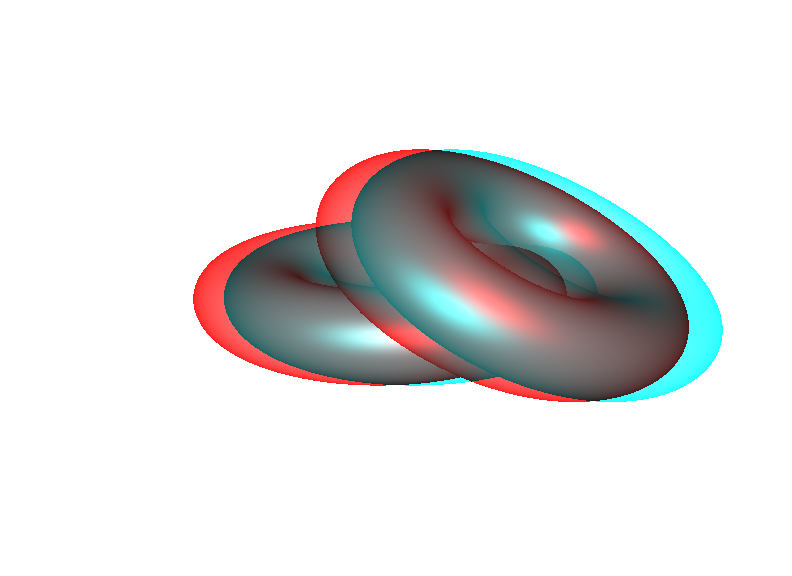
\includegraphics[scale=0.3]{photoshop.png}
	\caption{\label{fig:photoshop} Anaglyphe obtenu avec la méthode Photoshop \protect}
\end{figure}
		
% %ne pas oublier de mettre une référence à l'article

	Au niveau du résultat, on constate la présence de quelques d'artefacts notamment à l'écran sur des formes complexes avec beaucoup de détail. A l'impression, le rendu est plus agréable avec moins d'artefact. Globalement, cette méthode permet de voir rapidement la 3D sans trop fatiguer l'oeil.
%	--> la méthode la plus simple mais la qualité en couleur est mauvaise et il y a un peu de artefact
\subsubsection{La méthode des moindres carrés avec correction gamma}
%gamma -> prend en compte le support : écran
	Le deuxième algorithme implémenté est basé sur la méthode des moindres carrés présentée dans l'article \cite{algoDubois} par Eric Dubois. Dans cet article, comme David Romeuf l'explique \cite{explicationAlgoDubois} l'approche consiste à prendre en compte le spectre d'absorption des filtres des lunettes, la densité spectrale des sources primaires des écrans d'ordinateur et la sensibilité spectrale de l'œil humain, pour reproduire au mieux une image anaglyphe dont les couleurs sont proches de celles contenues dans l'image originale. Un exemple de rendu obtenu avec cette méthode est présenté dans la Figure \ref{fig:moindresCarres}.
	
	L'ensemble des couleurs visibles sur l'écran à travers les lunettes étant un sous ensemble de celui de l'écran, une transformation particulière est nécessaire et c'est pour cette raison que les moindres carrés interviennent dans la projection pour minimiser la distance entre les deux couleurs (celle obtenue et l'originale) dans le diagramme colorimétrique.
	
	L'algorithme implémenté met en \oe uvre une partie de la méthode décrite plus précisément dans cet article par Eric Dubois \cite{algoMoindreCarres} : notre algorithme utilise les matrices issues du calcul par projection avec la méthode des moindres carrés, et une correction gamma mais ne modifie pas la saturation.
	
	La correction gamma permet d'augmenter la luminosité, appliquée aux anaglyphes rouge-cyan le rouge est plus visible et l'impression de trois dimensions est renforcée. Cependant, l'augmentation de la luminosité implique une réduction des contrastes et peut résulter en une image avec les détails peu soignés.

\begin{figure}[h]
	\centering
	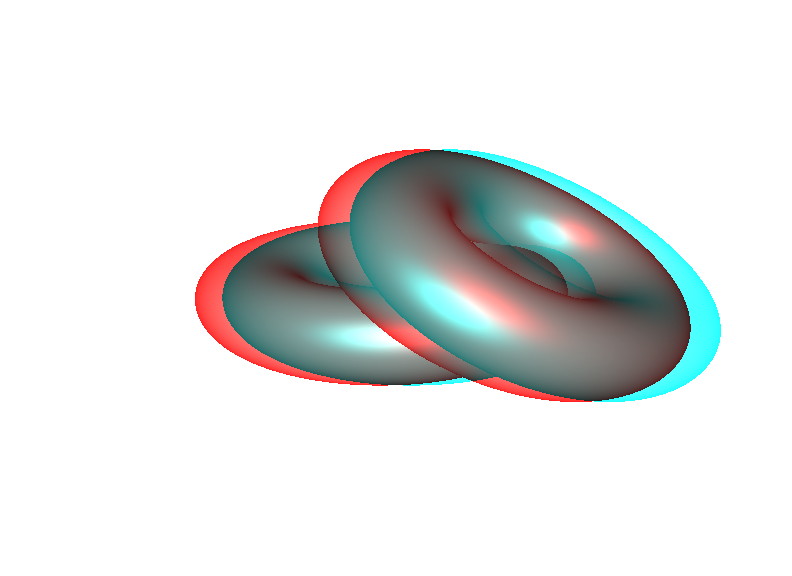
\includegraphics[scale=0.3]{moindreCarres.png}
	\caption{\label{fig:moindresCarres} Anaglyphe obtenu avec la méthode des moindres carrés \protect}
\end{figure}
	
	On constate qu'il y a très peu d'artefact et la 3D est de meilleure qualité que pour la méthode Photoshop. Toutefois, la qualité en couleur est légèrement perdue et les détails de l'image sont peu visibles. 
	

\subsubsection{Comparaison des différents algorithmes}

En comparant les algorithmes, il semblerait que pour une scène contenant un ou des objets simples % %REF FIGURE DOGNUTS
, la méthode Photoshop soit la plus efficace avec une impression de trois dimensions bien visible et peu d'artefacts. En ce qui concerne les objets plus complexes tels que % %REF FIGURE HAPPY
les détails se perdent avec la méthode Photoshop alors qu'avec la méthode de Dubois tous les détails sont conservés dans l'image anaglyphe résultat. 
% %dognuts photshop & dubois
% %happy photoshop & happy dubois 

Cependant, après plusieurs comparaisons des images (et ce par différentes personnes) la correction gamma employée dans la méthode de Dubois fatiguerait plus vite les yeux que la méthode Photshop.

Par ailleurs, il a aussi été observé que l'utilisation de l'anti-aliasing combiné aux algorithmes de génération d'anaglyphe, peut permettre de renforcer l'impression de trois dimensions dans certains cas. Cependant, l'anti-aliasing aura aussi pour effet de perdre beaucoup de détails comme la figure REF le montre avec un comparatif d'algorithmes avec et sans utlisation d'anti-aliasing. 
% %happy anti-aliasing dubois &  happy dubois (sans anti-aliasing)

Un autre point remarqué lors des différentes observations est la fatigue des yeux provoquée par la vision des anaglyphes et celle-ci varie selon les algorithmes. Il semblerait que l'algorithme de Dubois fatiguerait plus vite les yeux et que l'utilisation d'anti-aliasing rendrait la perception plus agréable et donc moins fatiguante. 
%l'algo dubois avec saturation -> la diminution de saturation, atténue trop les couleurs : moins bonne 3D mais moins fatiguant pour les yeux 

\subsubsection{L'impression des anaglyphes}
Dans ce projet, les anaglyphes générés par le logiciel étaient destinés à être visionnés sur écran mais aussi être imprimés sur papier. Le système de colorimétrie d'une imprimante est en CMJN (Cyan Magenta Jaune Noir) et son ensemble de couleur est plus réduit que celui des écrans. 

% %INSERER Diagramme comparatif pour illustrer ?

Par conséquent, le problème pour l'impression réside tout d'abord en la conversion du système RVB au CMJN. Tout comme l'algortihme de Dubois avec la méthode des moindres carrés \cite{algoDubois}, il faudrait pouvoir convertir en CMJN en essayant d'obtenir une couleur qui sera la plus proche possible de celle en RVB. 

Lorsque ce problème a été exposé en réunion avec les clients, il nous a été spécifié que nous n'avions pas besoin d'implémenter des méthodes pour améliorer l'impression. 

Par ailleurs, la conversion n'est pas le seul problème puisque comme expliqué avec l'article Andrew J. Woods et Chris R. Harris \cite{anaglypheDefaut}, le support d'affichage est aussi important : dans ce cas, le type de papier rentre aussi en compte dans la qualité de l'anaglyphe.

Finalement, la qualité de l'impression d'un anaglyphe dépendant trop des réglages en amont et du matériel utilisé, aucun algorithme particuliers n'a été implémenté. Cependant, nous avons choisi de laisser la possibilité à l'utilisateur de paramètrer le rendu de l'anaglyphe en modifiant la translation, la correction gamma, ajoutant de l'anti-aliasing afin que chacun puisse trouver de bons paramètres pour l'affichage à l'écran et à l'impression.
%peut etre en conclu de cette partie anagyphe ? AJOUTER : certains fatiguent plus les yeux que d'autres

  \subsection{Choix des algorithmes d'autostéréogrammes}
    Les deux algorithmes implémentés ont un squelette très similaire ; il s'agit, à partir de la carte des profondeurs, de lier deux par deux les pixels de l'image générée puis de colorier chaque paire de la même couleur.

  Les deux algorithmes sont dotés d'une technique anti-surfaces cachées (implémentée différemment dans les deux cas). D'autre part, ils supportent tous deux l'utilisation de textures 
  
  \subsubsection{Algorithme de base (Witten, Inglis, Thimbleby)}

  Cet algorithme a été choisi pour sa simplicité qui le laisse tout de même fonctionnel ; il a été conçu à l'origine pour des autostéréogrammes aléatoires en noir et blanc (SIRDS) mais a été adapté ici à d'autres types de rendus.

  Les résultats obtenus sont cependant assez peu satisfaisants pour la représentation d'objets complexes, comme le montre la figure \ref{fig:autoste1} : l'image est assez plate, et l'objet en relief est fait de paliers superposés plutôt que d'avoir une surface lisse. De ce fait, représenter des détails ou des courbes est ardu. L'utilisation de textures peut permettre d'atténuer certains défauts visuels, mais pas de les effacer totalement.

\begin{figure}[h]
	\centering
	
\includegraphics[scale=0.3]{autoste1.png}
	\caption{\label{fig:autoste1} Rendu d'un autostéréogramme avec l'algorithme de Witten, Inglis et Thimbleby \protect}
\end{figure}

  \subsubsection{Algorithme de W. A. Steer}
  
  L'algorithme de W. A. Steer a été choisi à cause des nombreuses améliorations qu'il apporte par rapport à l'algorithme précédent. En effet, il utilise une méthode de suréchantillonnage de l'image : dans une première étape, un autostéréogramme $n$ fois plus large que l'image de base est construit puis les pixels sont fusionnés par groupes de $n$. Ces étapes permettent d'améliorer la résolution en profondeur de l'autostéréogramme.
  
  Cet algorithme est plus lent que le précédent à cause du suréchantillonnage, mais les résultats obtenus sont nettement plus agréables à regarder car la résolution en profondeur est meilleure : l'image apparaît plus profonde comme le montre la figure \ref{fig:autoste2}. De plus, l'utilisation conjointe d'une texture et du suréchantillonage lisse l'image finale ; on n'y retrouve plus les ``paliers'' des résultats précédents. Ces paliers peuvent être visibles si le rendu choisi est de type aléatoire, mais ils sont beaucoup plus nombreux et rapprochés.

\begin{figure}[h]
	\centering
	
\includegraphics[scale=0.3]{autoste2.png}
	\caption{\label{fig:autoste2} Rendu d'un autostéréogramme avec l'algorithme de W. A. Steer \protect}
\end{figure}

  \subsection{Réalisation du projet}
  \subsubsection{Présentation générale de la réalisation}
\paragraph{}
La partie Réalisation de ce projet se sera étalée sur les mois de Décembre, Janvier, Février et Mars. Grâce à la réflexion effectuée durant la phase de rédaction du cahier des charges, nous avons pu aborder notre projet avec une idée claire des priorités.

\paragraph{}
L'implémentation des algorithmes de rendus étant centrale au projet, nous avons dès le début de la réalisation mis en place deux équipes de deux personnes pour les deux rendus principaux : les anaglyphes et les autostéréogrammes. Les folioscopes quand à eux ne demandaient pas d'algorithmes particulier, si ce n'est la manipulation de la caméra vis à vis de la scène qui allait être mise en place grâce à la troisième équipe.

\paragraph{}
En effet, notre troisième équipe, constituée des trois derniers membres, a pu continuer de travailler sur le prototype généré lors de la phase du cahier des charges. Il a ainsi été amélioré pour intégrer les parseurs de fichiers objets qui allaient être nécessaires pour la génération des éléments de la scène, et rendre plus agrèable la manipulation des objets et les déplacements dans la scène.

\paragraph{}
Malheureusement, l'implémenation des algorithmes s'est révélée plus longue que nous l'avions initialement prévue. Le mois prévisionnel n'étant pas uniquement dédié au projet PFA, les différents imprévus et un jugé peut-être trop léger de la difficulté que représentait cette étape ont engendré un retard par rapport au prévision. De plus amples explications seront données dans la partie ``Difficultés rencontrées'' de ce rapport. 
Au final, les recherches concernant les autostéréogrammes et anaglyphes auront pris deux mois et demi au lieu d'un seul. Deux mois ont servi à la réalisation de tests sur des prototypes pour évaluer la qualité des rendus, le demi mois concerne l'intégration au reste du logiciel avec d'autres tests pour trouver les réglages optimaux des algorithmes.

\paragraph{}
En parallèle, la troisième équipe, appuyée parfois par des membres des autres groupes en cas de besoin, a continué d'avancer sur la partie Scène du logiciel. L'implémentation de certaines manipulations de scène (déplacements de la caméra ou des objets notamment) auront parfois étaient plus rapides que prévu, mêmes si quelques retours en arrière ont été nécessaires au milieu du projet comme nous l'expliqueront dans la partie ``Difficultés rencontrées''.

L'ordre chronologique initialement prévu dans le diagramme de Gantt n'aura finalement pas toujours été respecté. Par exemple, la différence de travail entre l'ajout d'un objet dans la scène et l'ajout de plusieurs objets n'étant pas énorme, ces deux parties auront été effectuées simultanément. Il en est de même pour la sauvegarde automatique qui aura été ajoutée en même temps que la sauvegarde classique de la scène, ou encore pour les manipulations de la scène et de l'objet dont l'implémentation était grandement facilitée par l'utilisation de la bibliothèque OpenGL pour Qt.

\paragraph{}
Au final, la totalité des tâches prévues jusqu'au début du mois de Mars auront pu être effectuées dans les temps, nous laissant le mois de Mars pour l'intégration des algorithmes au logiciel, l'amélioration de certaines fonctionnalités, le développement de l'interface et la rédaction de ce rapport.



\subsubsection{Les algorithmes du logiciel}
\paragraph{}
Pour pouvoir permettre à l'utilisateur de notre logiciel d'obtenir des anaglyphes ou des autostéréogrammes il a fallu prospecter sur internet afin de trouver suffisamment d'articles scientifiques et de site traitant le sujet pour établir des comparaisons et choisir parmi toutes les solutions proposées celles qui offraient le meilleur résultat.

\paragraph{}
Cet exercice s'est révélé assez complexe car le travail de recherche qui s'y rapporte a été long, et il était parfois difficile de trouver les bonnes informations pour répondre à nos interrogations. Nos clients nous auront longuement accompagné dans notre travail de recherche, et nous aurons conseillé sur des outils pour trouver des articles pertinants. Cette partie ``Recherche de l'existant'', qui s'est principalement déroulée durant la phase de rédaction du cahier des charges, aura été formatrice car elle nous aura appris à utiliser les bons outils (comme google scholar) et les bons mots-clés pour rendre nos recherches fructueuses.

\paragraph{}
Une fois les algorithmes choisis, l'utilisation de cartes de profondeurs et de paires d'images stéréoscopiques trouvées sur Internet ont permis de faire des tests sur des prototypes indépendants du logiciel final. Leur implémentation s'est faite durant le dernier du projet. Il a donc fallu définir les entrées et les sorties pour chaque méthodes, afin de satisfaire l'architecture du projet et faciliter par la suite l'intégration d'autres algorithmes dans le logiciel.
La partie gérant la scène est considérée comme une boite noire avec laquelle les algorithmes de rendus intéragissent. Seul les entrées et les sorties sont connues ce qui permet de garantir la modularité de la partie rendue. 

\paragraph{}
Malgré les tests de pré-intégration fait sur les prototypes, des problèmes ont été rencontrés au moment de l'implémentation. Par exemple, pour les anaglyphes, le passage à l'utilisation de prises de vues issues de scène non-réelle donnait des résultats de moins bonnes qualités. Trouver le bon angle pour les couples d'images stéréoscopiques n'était pas non plus une chose aisée.
Ce problème ne provenait finalement pas de l'algorithme en lui-même, mais de la scène utilisée. En effet, les tests effectués sur des images n'avaient pas de contours aussi nets que les objets de la scène, et le rendu obtenu était correct. Toutefois, les fichiers d'extension OBJ et PLY sont constitués de triangles, et leurs bords sont très marqués, ce qui cause parfois une erreur au moment de la génération de l'anaglyphe. Une solution possible pour régler ce problème aurait été de rendre les contors des objets moins abruptes, mais cette solution n'a pas été implémentée dans notre logiciel.

\paragraph{}
Au final, le travail sur les algorithmes fut très enrichissant car bien plus théorique que les autres parties du projet. La recherche et la compréhension des articles est une part plus importante du travail que leur intégration au projet. D'autant plus que tous les articles ne présentaient pas dans le détail leurs solutions, ce qui obligeait à faire des recherches supplémentaires pour trouver comment s'y prendre. L'obtention d'un rendu à partir de la scène est montré dans la figure \ref{figure:screenRendu}.

\begin{figure}[h]
	\centering
	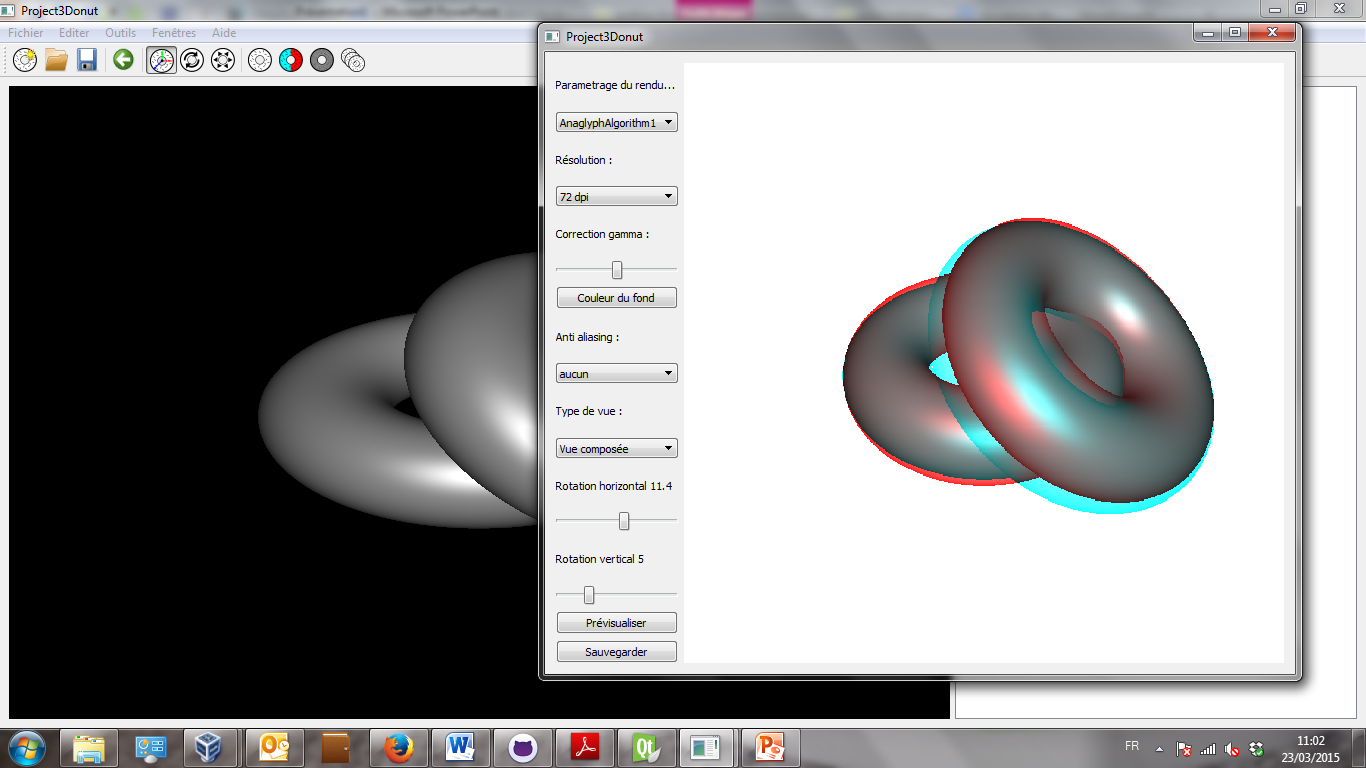
\includegraphics[scale=0.4]{rendu.png}
	\caption{\label{fig:screenRendu} Obtention d'un anaglyphe dans le logiciel \protect}
\end{figure}

\subsubsection{La manipulation de la scène}
\paragraph{}
Grâce à la rédaction du cahier des charges, les notions de scène en trois dimensions, de caméra et d'objet avait été acquise par notre équipe avant la phase d'implémentation. Un premier prototype de la scène, présenté dans la partie Cahier des charges, aura permis une première manipulation de ces notions et des bibliothèques Qt et OpenGL pour Qt afin de créer une première scène constituée d'un première objet. Les manipulations premières de la scène, notamment la rotation de la caméra tout autour de la scène, auront ainsi été mise en place pour pouvoir juger des capacités des bibliothèques, et déterminer la faisabilité de nos objectifs.

\paragraph{}
Dès la fin du cahier des charges, la scène aura été grandement modifiée. Les parseurs auront été finalisés pour pouvoir charger l'ensemble des fichiers objets demandés par les clients, et le stockage des objets de la scène aura été implémenté de telle façon que la gestion de plusieurs objets dans la scène a directement été opérationnelle. 

D'autres fonctionnalités, relatives à la scène et demandées par le cahier des charges, ont été implémentées peu à peu au cours de la phase de réalisation du projet. Au niveau de la scène, les rotations autour de la scène sont toujours possibles, ainsi qu'une fonction de zoom pour s'approcher ou se reculer de la scène. Au niveau des objets, la sélection d'un objet est possible soit en cliquant directement sur l'objet avec le bouton droit de la souris, soit en le sélectionnant dans la liste des objets donnée sur la fenêtre principale du logiciel. Une fois un objet choisi, on peut le déplacer, le faire tourner, modifier sa taille, sa couleur, ou encore le supprimer.

\paragraph{}
Grâce à l'ensemble des manipulations à mettre en place sur la scène, notre équipe a pu se familiariser et apprendre à utiliser les bibliothèques Qt et OpenGL pour Qt. De plus, la communauté Internet de la bibliothèque Qt nous aura été fort utile car elle aura permis de trouver des réponses à d'éventuels problèmes rencontrés, voire de poser des questions dans des cas particuliers.

\paragraph{}
La fenêtre principale du logiciel est montrée dans la figure \ref{fig:screenScene}.

\begin{figure}[h]
	\centering
	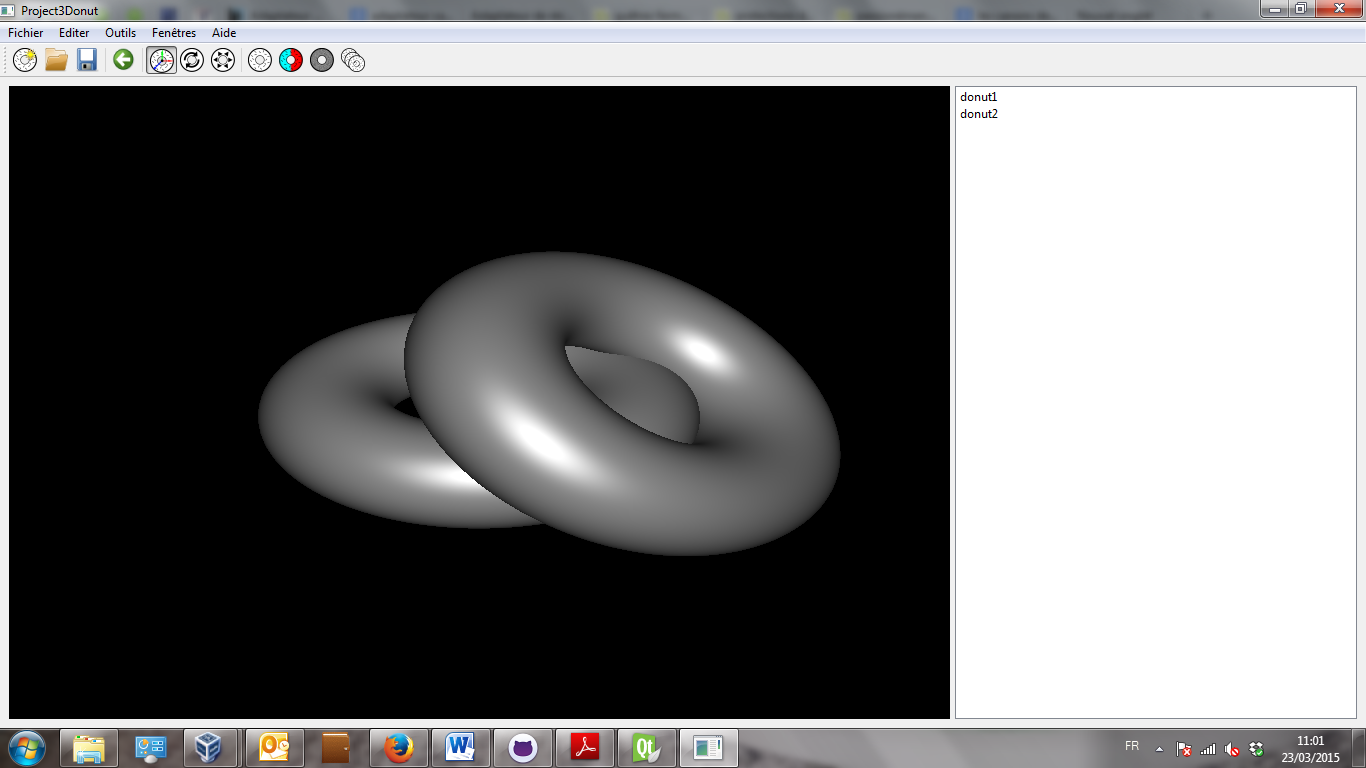
\includegraphics[scale=0.4]{Scene.png}
	\caption{\label{fig:screenScene} Visualisation de la scène dans le logiciel \protect}
\end{figure}

\subsubsection{Les sauvegardes et chargement de la scène}
\paragraph{}
Pour satisfaire la portabilité du logiciel, le nombre de bibliothèques utilisées devait être le plus faible possible. Fort heureusement, la bibliothèque Qt, portable sur la plupart des plateformes, propose une grande quantité de fonctionnalités, y compris le module QtXml qui permet la lecture et le découpage d'un fichier XML. Au cours de la phase de rédaction du Cahier des charges, nous avions mis au point un prototype de fichier XML pour permettre la sauvegarde et le chargement de la scène, que nous avons pu utiliser comme nous l'avions prévu grâce à Qt. Un exemple de fichier utilisé pour le chargement d'une scène effective dans notre logiciel, nommé 'MaScene.xml', est donné en Annexe.

[ANNEXE XML]

\paragraph{}
La sauvegarde d'une scène consiste principalement à écrire dans un fichier texte, en respactant le format souhaité par le format XML et en récupérant les bonnes informations des Objets et de la Caméra de la scène. Toutefois, deux types de sauvegarde ont été mises en place : une sauvegarde manuelle et une sauvegarde automatique.

La sauvegarde manuelle s'effectue de la même façon que dans la plupart des logiciels. A la demande de l'utilisateur, le logiciel va lancer une sauvegarde dans un fichier dont le nom est donné, et une fois que celle-ci sera achevée l'utilisateur pourra recommencer à travailler sur sa scène.

Pour la deuxième sauvegarde, nous avons dû utiliser nos connaissances acquises au cours des enseignements de Programmation Système et de Système d'Exploitation. Nous avons en effet vu d'une part comment utiliser des Threads, et d'autre part qu'un Thread en train de dormir ne demande pas d'intervention du processeur. Nous avons ainsi mis en place la création d'un Thread dès l'ajout d'un premier objet dans une scène, et ce Thread va dormir durant un certain temps avant d'effectuer une sauvegarde automatique puis de se rendormir. Cette attente passive permet ainsi de ne pas gaspiller de temps du processeur, et de sauvegarder les avancées de la scène en cas d'arrêt non souhaité du logiciel. De plus, le temps d'attente entre deux sauvegardes automatiques peut être choisie par l'utilisateur grâce aux paramètres du logiciel.

\paragraph{}
La difficulté principale du chargement de la scène est de s'assurer de la validité du fichier XML passé en paramètre. Ainsi, de nombreuses vérifications, au fur et à mesure de la lecture du fichier, sont nécessaires afin de pouvoir créer une scène fonctionnelle. La bibliothèque QtXml aura été assez simple d'utilisation, et le chargement aura donc pu être rapidement mis en place, tout d'abord en parallèle du projet pour s'assurer que seuls les fichiers XML valides sont acceptés, puis après intégration pour s'assurer de l'appel des constructeurs et de la génération de la scène souhaitée.

\paragraph{}
L'utilisation du module QtXMl aura toutefois posé problème avec l'utilisation de CMake. En effet, la plupart des informations données sur Internet permette l'utilisation de ces modules avec QMake, et l'intégration est alors relativement simple. Pour l'intégrer à CMake, il aura fallu comprendre précisément le fonctionnement de CMake et trouver les bons noms de paquetages à intégrer afin que le module puisse être utilisé dans le logiciel.

\subsubsection{Architecture finale du projet}
\paragraph{}
L'architecture prévisionnelle de notre projet n'aura que peu été modifiée au fil de notre projet. La structure principale du projet est resté la même, avec les différents paquetages initialement prévus, mais comme le montre la figure \ref{fig:archi}, le Chargeur n'est plus le point d'entrée du paquetage Scene.

\begin{figure}[h]
		\centering
                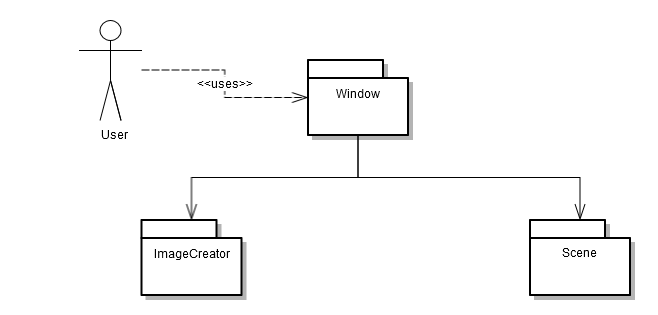
\includegraphics[scale=0.5]{paquetages.png}
		\caption{\label{fig:archi} Diagramme des paquetages en fin de projet \protect \footnotemark}
\end{figure}
\footnotetext{Réalisé grâce au logiciel Gliffy : \url{www.gliffy.com}}


Le paquetage Création tel que présenté dans la figure \ref{fig:creation} n'a pas connu de modifications particulières. En effet, les dépendances entre les différentes classes étaient très importantes pour l'extensibilité du logiciel. Toutefois, de nouvelles classes ont été ajoutées, pour permettre la création des images et des folioscopes.

\begin{figure}[h]
		\centering
                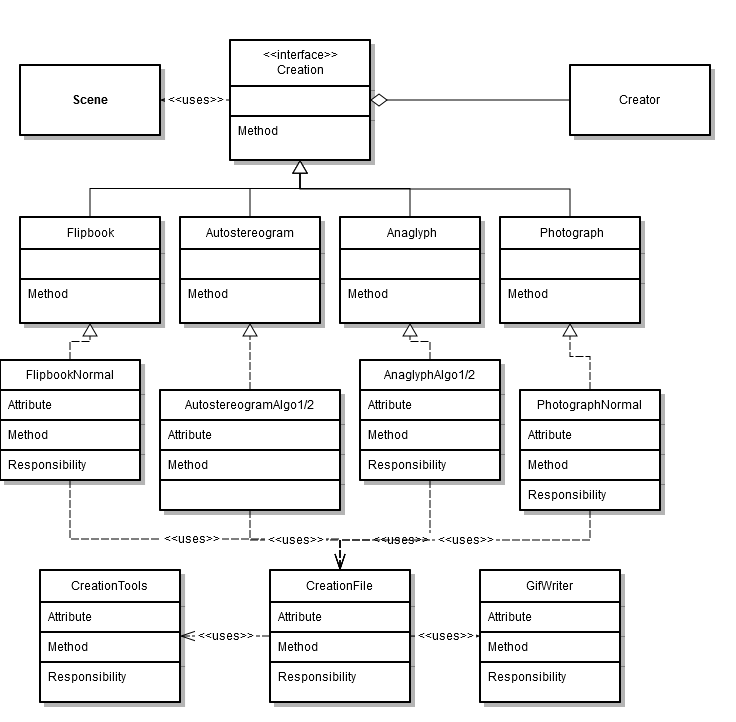
\includegraphics[scale=0.5]{f_creation.png}
		\caption{\label{fig:creation} Paquetage Creation en fin de projet \protect \footnotemark}
\end{figure}
\footnotetext{Réalisé grâce au logiciel Gliffy : \url{www.gliffy.com}}


Le paquetage Interface contient les classes principales permettant la génération des fenêtres du logiciel. Le logiciel QtCreator aura été utilisé pour aider à la génération des ces fichiers sources.

Le paquetage Scene a quant à lui été modifié. Si nous avions initialement prévu que ce soit le Loader qui se charge de créer la scène et les objets qui s'y trouvent, c'est finalement la classe Scene en elle-même qui est devenue le point d'entrée du paquetage Scène. Elle se charge ensuite de transférer les informations nécessaires au Loader pour qu'il se charge de charger les objets. Le paquetage final de la Scene est présenté dans la figure \ref{fig:scene}.

\begin{figure}[h]
		\centering
                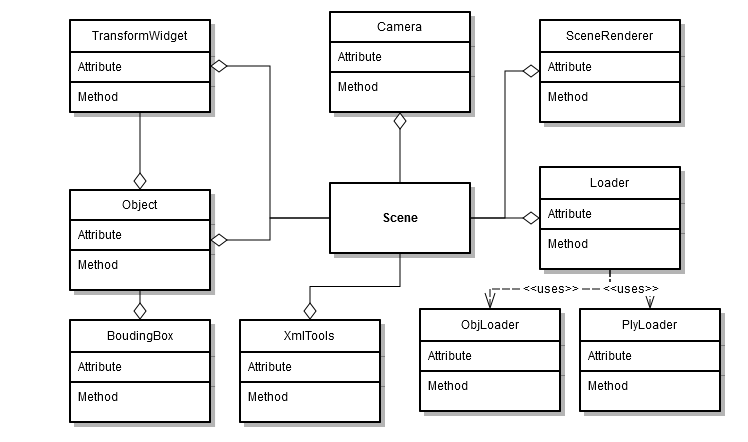
\includegraphics[scale=0.5]{f_scene.png}
		\caption{\label{fig:scene} Paquetage Scene en fin de projet \protect \footnotemark}
\end{figure}
\footnotetext{Réalisé grâce au logiciel Gliffy : \url{www.gliffy.com}}

  \subsection{Test des fonctionnalités}
  Explication des tests réalisés pour valider les besoins fonctionnels/non fonctionnels du cahier des charges

\paragraph{}
Pour valider la réalisation des besoins fonctionnels et non fonctionnels présentés dans le cahier des charges, une série de tests a été effectuée sur le logiciel.

\paragraph{}
Concernant les besoins fonctionnels, nous avons manipulé le logiciel sous les différents systèmes d'exploitation envisagés, à savoir Windows et Linux.
Les différentes rotations de la caméra autour de la scène ont bien été implémentées, permettant à l'utilisateur de voir les objets qui y sont placés sous différents angles, et de s'en rapprocher ou de s'en éloigner grâce au zoom.
[TRANSLATION]
Les objets sont issus de fichiers d'extension OBJ version 3.0, ASCII, ou PLY, versions 1.0, ASCII et binare. Ceux-ci peuvent ensuite être sélectionnés un par un, en cliquant sur la scène ou sur son nom dans la liste des objets. L'utilisateur peut alors les déplacer grâce à des translations et rotations selon trois axes, et modifier leur taille. Ils pourront également être supprimés de la scène.
Enfin, les différents rendus prévus ont pu être obtenus à partir de la scène. Pour chacun d'entre eux, une nouvelle fenêtre est ouverte, proposant les paramètres modifiables pour la génération des photographies, anaglyphes, autostéréogrammes, et folioscopes. Pour chacun d'entre eux, on proposera une prévisualisation, et la possibilité d'enregistrer [LES IMAGES INTERMEDIAIRES ayant permis ce résultat, à savoir les vues gauche et droite pour les anaglyphes, la carte des profondeurs pour les autostéréogrammes, et chaque image du folioscope permettant d'obtenir un GIF animé.]    
[VERIFIER SI CEST OK]
[SAUVEGARDES]


\paragraph{}
Les tests des besoins non fonctionnels ont permis de valider la portabilité et la fluidité du logiciel. L'extensibilité du logiciel aura été permise par l'architecture du logiciel, qui a été présentée dans la partie Réalisation du projet.
Pour s'assurer de la portabilité du logiciel, nous avons manipulé le logiciel sous les différentes machines de notre équipe de programmeur, aussi bien sous Linux que sous Windows, avec ou sans carte graphique intégrée. L'ensemble des fonctionnalités précisées dans la paragraphe précédent ont été testées pour s'assurer de leur bon fonctionnement.
La fluidité du logiciel a été testée grâce au modèle happy.ply qui avait servi de modèle lors de la réalisation du cahier des charges. 
[SCREENS]
[RESULTATS WINDOWS/LINUX/CHIPSET]
[LOGICIEL DE TEST]

\paragraph{}
L'ensemble de ces tests auront permis de s'assurer de la conformité de notre projet au Cahier des charges. 

  \subsection{Difficultés rencontrées}
  \paragraph{}
	Ce projet s’inscrit dans le domaine de la synthèse d’images et de la visualisation de modèles en trois dimensions. Depuis le quinzième siècle, grâce à la peinture, la perspective apparaît sur des supports en deux dimensions. Aux XIXème et XXème siècles, l’utilisation de stéréoscopes, tel que le stéréoscope de Holmes, permettait la visualisation de relief à partir de deux images planes et d’un dispositif optique. Dans la deuxième moitié du XXème siècle, l’utilisation du numérique permet de modifier les images et d’obtenir une meilleure visualisation de la profondeur sur des supports en deux dimensions. 

\paragraph{}	
	On peut ainsi créer des anaglyphes, des autostéréogrammes ou des flipbooks, qui sur papier ou sur écran permettent d’apercevoir la profondeur d’une scène grâce à des techniques adaptées. Ces différents rendus seront présentés plus tard dans ce cahier des charges. De nos jours, il existe également des logiciels, tels que Meshlab et Blender qui sont gratuits, open source et permettent d’ores et déjà la visualisation en trois dimensions sur un écran. L’utilisateur peut tourner autour d’un objet et le voir sous tous ses angles grâce à un ensemble de projections successives autour de l’objet.

\paragraph{}
	On appelle synthèse d’image l'ensemble des techniques qui permettent de visualiser des objets en trois dimensions en perspective sur un écran d'ordinateur, en tenant compte de lumières et de textures appliquées à l'objet. Il existe un grand nombre de techniques et les résultats obtenus peuvent eux aussi varier (perspective isométrique, perspective conique...). Nous nous préoccupons par la suite de la perspective conique, dite aussi vue naturelle. 

\paragraph{}
	Bien souvent, la synthèse d'image utilise le principe de scène. Il s'agit d'un espace à trois dimensions dans lequel des objets peuvent être placés. Ces derniers sont décrits par un ensemble de points disposés dans l'espace.

\paragraph{}
	Pour pouvoir observer la scène et les objets, il est nécessaire de demander à l'ordinateur de les modéliser, c'est-à-dire d'afficher un rendu qui correspondrait à une vision de cette scène si elle était réelle. Pour cela, la machine simule le point de vue de l'utilisateur à l'aide d'une « caméra ». A partir de cette scène en trois dimensions, la caméra peut réaliser des projections ou photographies permettant de créer des anaglyphes, autostéréogrammes ou flipbooks. Plusieurs méthodes de projection existent, mais seule celle par matrice de projection sera utilisée.

\paragraph{}
	Ces matrices sont décrites à l’aide de coordonnées homogènes. Celles-ci ont été introduites afin que l’ensemble des transformations de type rotation, translation et homothétie puissent être écrites sous forme de matrice. Ainsi, le produit des matrices de transformation peut être calculé en amont pour pouvoir appliquer la matrice de la transformation résultante à l’ensemble des points de l’objet sans avoir à recalculer le produit pour chaque point.

\paragraph{}
	Pour pouvoir visualiser un modèle 3D il faut prendre en considération la lumière et sa réflexion sur l’objet. Si une sphère rouge était représentée dans un espace avec uniquement une lumière ambiante, il n’en ressortirait qu’un disque rouge, sans relief. En effet, la lumière ambiante atteint l’objet de la même façon en tout point. On ne peut donc pas savoir depuis un plan fixe s’il s’agit d’un objet en deux ou en trois dimensions. Si maintenant une lumière est ajoutée dans l’espace où est situé l’objet, celle-ci ne va pas atteindre tous les points de l’objet de la même façon. Elle sera plus faible sur un point plus éloignée, voire inexistante sur un point caché. En tenant compte de cette lumière, on peut obtenir une image comme présentée sur la figure \ref{fig:sphère}.

\begin{figure}[h]
	\centering
	
\includegraphics[scale=0.3]{boule.png}
	\caption{\label{fig:sphère} Application d’une lumière diffuse à une sphère rouge \protect \footnotemark }
\end{figure}
\footnotetext{http://linut.free.fr/omgspl0kuberwebloglolz0r/?2010/02/01/93-raytracer-que-la-lumiere-soit}

\paragraph{}
	Pour la création d’un anaglyphe, deux images espacées par une petite distance (qui correspond à la distance entre les deux yeux par exemple) sont générées. La composante rouge de l’une de ces images et la composante bleue de l’autre sont gardées et ensuite superposées dans une même image. Cette image est ensuite transformée en une image Rouge-Cyan, qui peut être visualisée à l’aide de lunettes Rouge-Bleue : l’image apparaît en trois dimensions.

\paragraph{}
	Pour la création d’un autostéréogramme, une image permettant d'observer un objet en relief par vision parallèle est générée. Cette image est obtenue à partir d'une texture de base ou de points aléatoires pour l'image de fond.

\paragraph{}
	Pour la création d’un flipbook, plusieurs images sont prises à intervalles réguliers par une caméra suivant un trajet prédéterminé dans ou autour de la scène. Le flipbook est visualisable en faisant rapidement défiler ces images tout en respectant l’ordre des prises de vue. Ce flipbook peut être transformé en GIF pour obtenir une visualisation animée des images.

  \subsection{Bilan technique}
  \paragraph{}
Au final, l'ensemble des manipulations de la scène et de ses objets qui avaient été promises dans le cahier des charges ont été implémentées. De même, l'ensemble des rendus prévu est générable à partir de la scène, deux algorithmes de génération sont proposés pour les autostéréogrammes et trois pour les anaglyphes.

\paragraph{}
Au niveau des besoins non fonctionnels, la portabilité aura été presque respectée malgré l'utilisation des shaders qui auraient pu poser problème sur certaines machines. Grâce aux nombreux modules proposés par la bibliothèque Qt, portable et très complète, des solutions auront été trouvées pour l'ensemble des modules et des cas d'utilisation sans avoir à sacrifier de fonctionnalité pour permettre l'utilisation du logiciel aussi bien sous Windows que sous Linux. La seule exception reste la machine Windows XP 32 bits qui avait été prévue lors de la phase du Cahier des Charges, car cette machine n'a pas pu être testée à cause de difficultés avec les outils utilisés, notamment CMake.

\paragraph{}
Bien que l'indication ne soit pas donnée dans le logiciel, l'utilisation de Project3Donuts en parallèle de l'utilisation du logiciel Fraps\footnotemark nous a permis de vérifier la fluidité du logiciel. Grâce notamment aux modèles 'happy.ply' et 'blade.ply' présentés dans le cahier des charges, les valeurs de frames par seconde données dans le cahier des charges ont été largement validées sur l'ensemble des machines.
\footnotetext{\url{http://www.fraps.com/}}
\paragraph{}
Enfin, la maintenabilité du logiciel sera également possible grâce au choix des outils et à l'architecture du projet. 
Tout d'abord, l'utilisation de Qt5, qui est actuellement la plus récente version de Qt, laisse envisager que le logiciel pourra être utilisé longtemps sans avoir à migrer vers une nouvelle version de la bibliothèque. Ensuite, l'utilisation de OpenGL ES 2.0, qui est la version d'OpenGL de base avec Qt5, pourrait éventuellement permettre de générer une application mobile du logiciel. 
L'architecture a également été pensée pour permettre cette maintenabilité. En effet, la présence des différents rendus et de plusieurs algorithmes pour chaque rendu montre bien qu'il est aisé d'en ajouter de nouveau.

\paragraph{}
Ce bilan positif montre qu'une très grande majorité des besoins fonctionnels et non fonctionnels ont pu être mis en place dans notre logiciel. Nous espérons que ce projet sera réutilisé et maintenu, puisqu'il a été conçu dans cette optique. Il sera éventuellement possible de créer une application mobile à partir du code existant, ou d'ajouter et de tester d'autres algorithmes ou d'autre rendus possibles à partir d'une scène en trois dimensions. Nous espérons également que nos clients auront été satisfaits du travail réalisé et du logiciel final. 


  \subsection{Bonus d'implémentation et possibilités d'évolution}
  \paragraph{}
Dans la dernière phase de notre implémentation, nous avons pu ajouter quelques fonctionnalités pour améliorer le logiciel et le rendre plus proche de certains logiciels plus professionnels.

Tout d'abord, à la demande de nos clients, nous avons ajouté la possibilité d'annuler la dernière action effectuée quand celle-ci agit sur l'état d'un objet, son ajout ou sa suppression. Grâce à un stockage de lambda-expression, permises par le C++11, chaque action est enregistrée. Lorsque l'utilisateur utilise le raccourci clavier Control+Z, la dernière fonction ajoutée au vecteur de lambda-expression est récupérée, et l'inverse de l'action est effectuée.

Nous avons également implémenté des fonctionnalités pour coller aux préférences de l'utilisateur. Par exemple, l'utilisateur peut choisir le durée qu'il souhaite imposer entre deux sauvegardes automatiques du logiciel, la couleur du fond de la scène, ou encore l'emplacement de la barre verticale dans laquelle sont listés les objets présents sur la scène. Il peut également modifier les raccourcis clavier pour les personnaliser.

La couleur des objets est également devenue un paramètre modifiable. Après sélection d'un objet, l'utilisateur peut, grâce au menu déroulant prévu à cet effet, en modifier la couleur. Cette modification sera effective dans la scène et lors des rendus, mais ne sera pas sauvegardée avec les autres caractéristiques de l'objet.

Un repère a été placé dans la scène pour que l'utilisateur puisse à tout moment se repérer par rapport aux trois axes géométriques.

Enfin, après avoir pris conscience que le rendu de base d'OpenGL présentait des problèmes au niveau des bords des objets. De l'anti-aliasing a été mis en place lors de la génération des rendus. Cela a permis d'augmenter la qualité des anaglyphes, en réduisant les artefacts au niveau des bordures.


\paragraph{}
Faute de temps, d'autres améliorations éventuelles du logiciel n'ont pas pu être mises en place, mais représentent d'éventuelles perspectives d'amélioration pour notre logiciel.

Ce projet a été conçu pour permettre son extensibilité, principalement au niveau des algorithmes et des possibilités de création de rendus divers. On pourrait alors réfléchir à implémenter de nouveaux algorithmes, existants ou à venir, pour tester et comparer leur qualité. On pourrait également imaginer d'autres rendus, comme un flipbook d'anaglyphes ou des autostéréogrammes dynamiques.

Bien que le logiciel permette à l'utilisateur de le personnaliser, certains raccourcis ou fonctionnalités n'ont pas été implémentés, comme la sélection multiple d'objets ou le clic droit sur un objet déjà sélectionné pour connaître d'éventuelles actions effectuables sur cet objet. Cette éventualité pourrait permettre de rendre le logiciel plus agréable à manipuler pour ses utilisateurs.

Un autre objectif potentiel serait le passage du logiciel sous un environnement MAC. Faute de machines de test, nous n'avons pas eu l'occasion de tester notre code avec ce système d'exploitation, mais nous pensons que la transition vers celui-ci pourrait s'avérer relativement simple.

Enfin, l'utilisation de la version 2.0 ES de la bibliothèque OpenGL offre la possibilité d'implémenter le logiciel sous d'autres plateformes, comme par exemple des tablettes graphiques ou des téléphones portables. On pourrait éventuellement imaginer prendre des photos d'une scène environnante et la transformer grâce à d'autres algorithmes en des anaglyphes ou des autostéréogrammes. 

\paragraph{}
Les possibilités d'évolution du logiciel Project3Donuts sont donc multiples, et nous espérons que celui-ci pourra être amélioré ou réutilisé par la suite dans de nouveaux projets.

  \newpage

  \section{Retour sur la gestion de projet}
  Dans cette partie, nous reviendrons plus en détails sur la partie gestion de projet de notre PFA, depuis sa préparation avec le cahier des charges jusqu'à sa réalisation.
  \subsection{Cahier des charges}
    acquis grâce au cahier des charges
  apprentissage de la rédaction / mise en forme
  compréhension du but
  objectifs fixés
  difficultés rencontrées

%	\paragraph{} 
%        Lors de notre premier rendez-vous, notre client a d'ores et déjà défini le format qu'il souhaitait pour le cahier des charges, et le contenu qui était essentiel pour lui. Il fallait ainsi présenter le domaine d'études et les connaissances actuelles sur des algorithmes de création d'anaglyphes, d'autostéréogrammes ou de folioscopes. Ensuite, le sujet était à redéfinir précisément, puis les besoins fonctionnels et non fonctionnels demandés par les clients pour ce logiciel, ainsi que les contraintes engendrées par ceux-ci. Enfin, il fallait présenter des prototypes permettant de répondre aux différents besoins ennoncés, quelques interfaces graphiques pour simuler l'utilisation du logiciel, et surtout réfléchir à l'architecture future du projet.

%\paragraph{}
%        La rédaction des parties Domaine et Etat de l'existant aura demandé de nombreuses recherches, notamment pour trouver des articles présentant des algorithmes de création d'anaglyphes et d'autostéréogrammes. 
%	L'étude du domaine aura permis de se familiariser avec le vocabulaire de la synthèse d'image et avec les différents rendus souhaités par nos clients. Des notions telles que la scène, la caméra, ainsi que la compréhension du fonctionnement des anaglyphes et des autostéréogrammes auront ainsi permis une meilleure immersion dans notre projet.

%	Les algorithmes relatifs aux anaglyphes concernent principalement le traitement des couleurs pour qu'aucun artefact n'apparaisse au moment de la visualisation finale. Pour les autostéréogrammes, le traitement d'une carte des profondeurs permet d'obtenir une image qui, lorsque l'on sait l'observer, fait apparaître un relief. Enfin, il n'existe pas d'algorithme particulier pour la génération de folioscopes. Seule une série de prises de vue d'une scène avec des angles d'observation proches peuvent permettre, si elles sont visualisées les unes à la suite des autres et suffisamment rapidement, de pouvoir imaginer un mouvement, et ainsi un relief.

%\paragraph{}
%        Les besoins fonctionnels et non fonctionnels d'un projet doivent impérativement être ciblés durant la phase de cahier des charges, car c'est grâce à eux que le contrat passé entre les clients et l'équipe de programmeurs pourra être exhaustif et protéger les deux parties contre d'éventuelles envies de modification au cours de la phase de réalisation. 
        

  \subsection{Diagramme de Gantt prévisionnel}
  \paragraph{}
Une fois le cahier des charges mis en place et l'accord des clients donnés, la première étape du projet consistait à réfléchir au diagramme de Gantt prévisionnel pour les trois mois destinés à la réalisation du projet.
La priorité était donnée aux algorithmes de réalisation des différents rendus, notamment les anaglyphes et les autostéréogrammes. Il fallait revenir sur les articles trouvés et présentés dans le cahier des charges pour s'approprier les méthodes présentés afin de pouvoir les retranscrire et approfondir les recherches pour peut-être trouvé d'autres algorithmes plus performant.
En parallèle, d'autres personnes pouvaient travailler sur une partie plus proche du logiciel finale, à savoir la manipulation de la scène ou encore les parseurs de fichiers pour le chargement des objets.
Une fois les manipulations premières de la scène effectuées, les travaux prioritaires étaient le chargement et la sauvegarde de la scène grâce à des fichiers d'extension XML, la création de prises de vue simples ou de folioscopes à partir de la scène et leur sauvegarde, et enfin l'assemblage complet du logiciel avec une interface d'utilisation permettant d'utiliser les différents modules.

\paragraph{}
Un récapitulatif du diagramme de Gantt prévisionnel du projet est donné page suivante.

\newpage
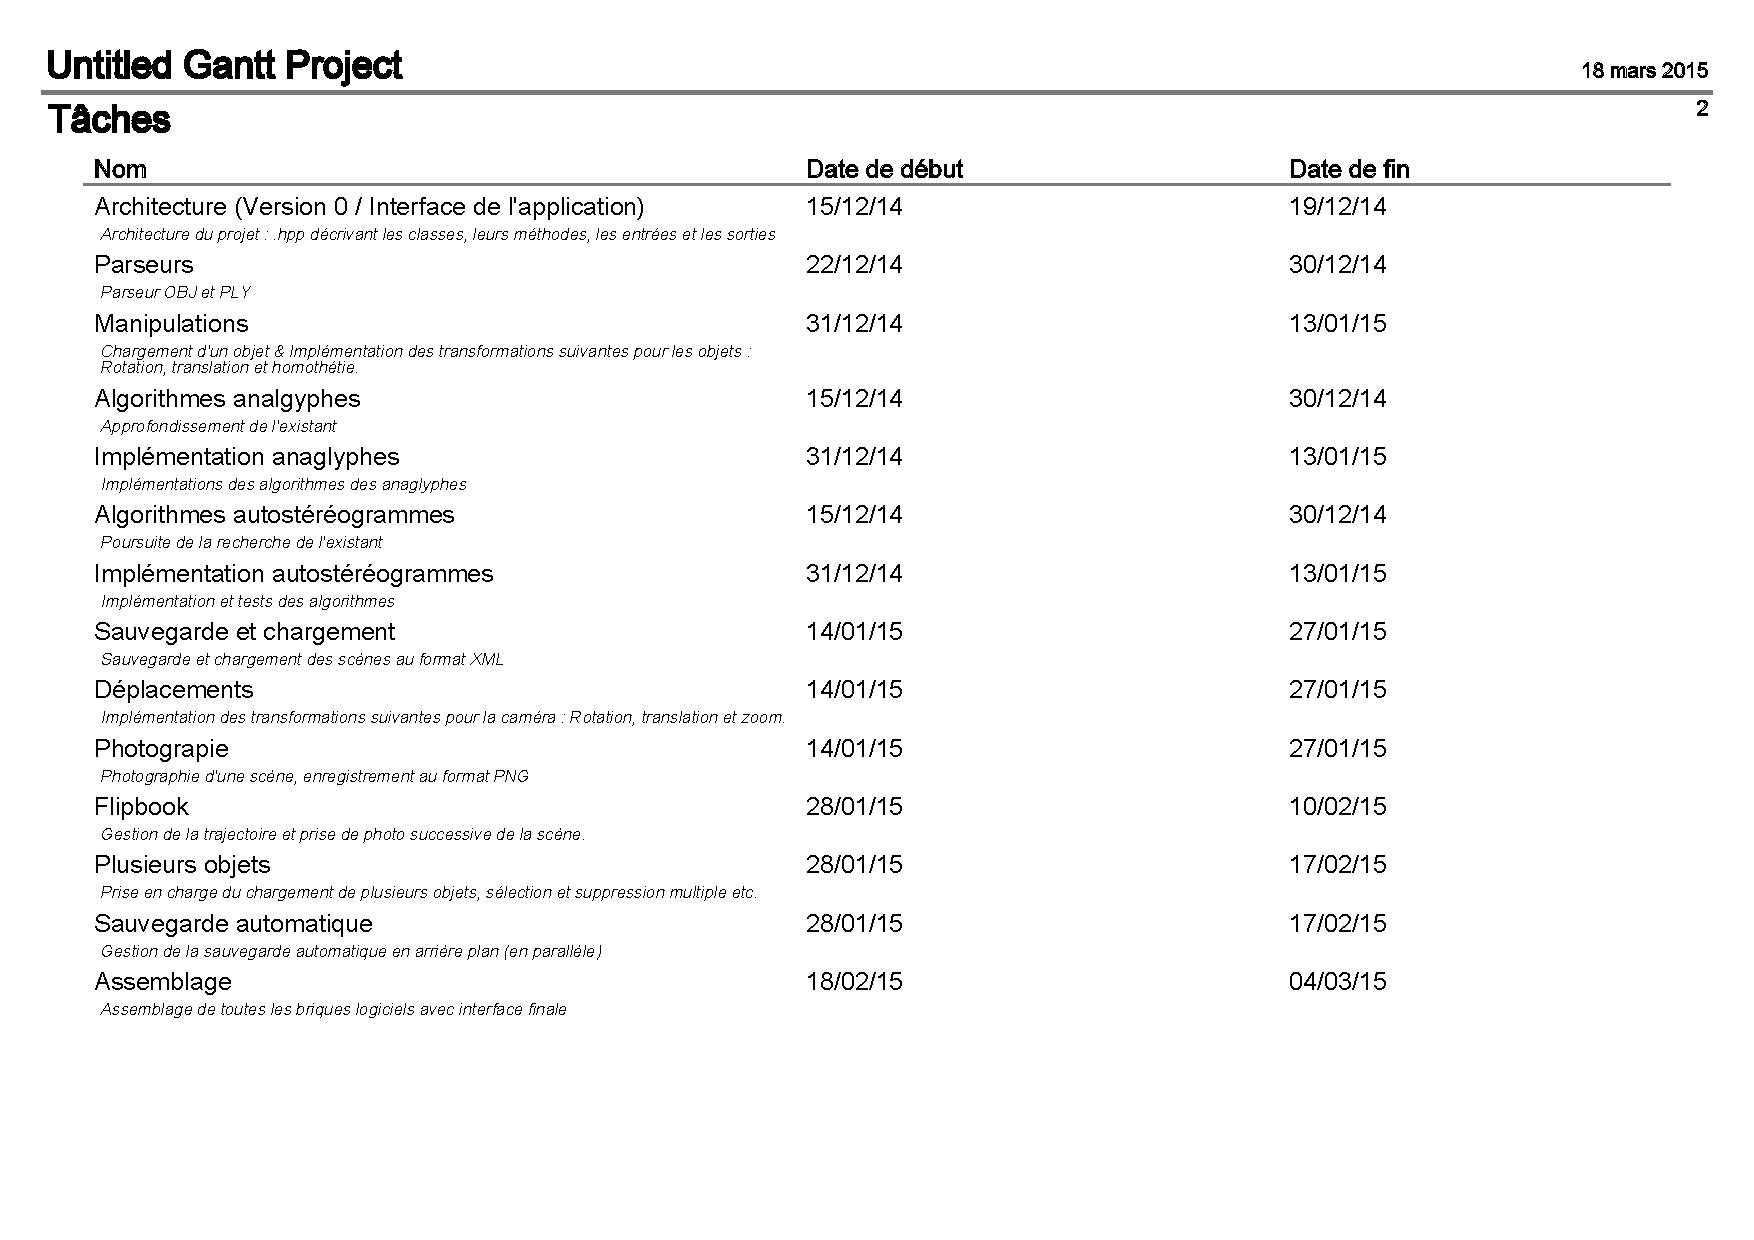
\includepdf[pages=1-1]{gantp.pdf}
\newpage

\paragraph{}
Pour déterminer les durées nécessaires à chaque partie de ce projet, nous avons dû réfléchir aux éventuelles recherches à réaliser au préalable, ainsi qu'à la complexité des tâches en les découpant en sous-parties. Nous avons également réfléchi aux éventuels examens qui auraient pu nous ralentir dans la réalisation en fonction des périodes.

\paragraph{}
Ainsi, pour une tâche telle que l'implémentation d'algorithme d'anaglyphes, il fallait dans un premier temps revenir et compléter les recherches faites sur l'état de l'existant. En effet, comme nous l'avons vu dans la partie présentation du projet, de nombreuses études ont été effectuées pour mettre en place des algorithmes plus ou moins performants capables de générer des anaglyphes. Une fois le choix des algorithmes effectués, l'implémentation de celui-ci en C++ pourrait être effectuée.
Au final, la période déterminée pour la recherche d'algorithmes et l'implémentation de ces algorithmes était d'environ un mois pour une équipe de deux personnes.

\paragraph{}
Un autre exemple de période déterminée est celle destinée à la sauvegarde et au chargement des scènes. Nous avions d'ores et déjà un fichier XML modèle sur lequel s'appuyer, ce qui a permis de passer rapidement à l'implémentation. La sauvegarde consistant simplement en une écriture dans un fichier, seul le chargement demandait des recherches pour déterminer la meilleure bibliothèque pour effectuer le découpage d'un fichier XML. La période déterminée pour cette tâche était de deux semaines pour une équipe de deux personnes.

  \subsection{Bilan final}
  \paragraph{}
Comme nous l'avons expliqué dans la partie Réalisation, le diagramme de Gantt a dû être remanié au fil de l'avancement du projet car certaines tâches, plus faciles que prévues, ont été anticipées alors que d'autres, posant plus de problèmes, ont été allongées.
Le diagramme de Gantt a été donné en Annexe.

\paragraph{}
La principale modification consiste ainsi en l'allongement de la période destinée à la recherche d'algorithmes pour les rendus et à leur implémentation. Les raisons de cette différence ont été expliquées dans la partie Difficultés rencontrées ci-dessus.
Les manipulations des objets et de la scène ont été effectuées plus rapidement que prévu, mais une période de retour en arrière à cause des shaders a été ajoutée, allongeant la période de travail sur le chargement et la sauvegarde de la scène qui a été momentanément interrompue le temps de régler ce problème.

\paragraph{}
Malgré ces débordements dans le temps, la réalisation du projet se sera achevée dans les temps, le dernier mois ayant permis d'intégrer les algorithmes au logiciel, de compléter et de parfaire des fonctionnalités.
Au final, l'ensemble des manipulations de la scène et de ses objets qui avaient été promises dans le cahier des charges ont été implémentées. De même, l'ensemble des rendus prévu est générable à partir de la scène, et deux algorithmes de génération sont proposés pour les autostéréogrammes et les anaglyphes alors qu'un seul avait été cité pour l'autostéréogramme dans le cahier des charges, et que seul le traitement de couleurs pour l'impression avait été initialement prévu pour m'anaglyphe (et pas la saturation).

\paragraph{}
Au niveau des besoins non fonctionnels, la portabilité aura été respectée malgré l'utilisation des shaders qui auraient pu poser problème sur certaines machines. Grâce aux nombreux modules proposés par la bibliothèque Qt, portable et très complète, des solutions auront été trouvées pour l'ensemble des modules et des cas d'utilisation sans avoir à sacrifier de fonctionnalité pour permettre l'utilisation du logiciel aussi bien sous Windows que sous Linux.

\paragraph{}
[FLUIDITE]

\paragraph{}
Enfin, la maintenabilité du logiciel sera également possible grâce au choix des outils et à l'architecture du projet. 
Tout d'abord, l'utilisation de Qt5, qui est actuellement la plus récente de Qt, laisse envisager que le logiciel pourra être utilisé longtemps sans avoir à migrer vers une nouvelle version de la bibliothèque. Ensuite, l'utilisation de OpenGL ES 2.0, qui est la version d'OpenGL de base avec Qt5, pourrait éventuellement permettre de générer une application mobile du logiciel. 
L'architecture a également été pensée pour permettre cette maintenabilité. En effet, comme le prouvent les deux algorithmes 


\paragraph{}
Ce bilan positif montre que l'ensemble des besoins fonctionnels et non fonctionnels ciblés dans le cahier des charges ont été implémentés avec succès. Nous espérons que ce projet sera réutilisé et maintenu, puisqu'il a été conçu dans cet optique. Il sera éventuellement possible de générer une application mobile à partir du code existant, ou d'ajouter et de tester d'autres algorithmes ou d'autre rendus possible à partir d'une scène en trois dimensions. Nous espérons également que nos clients auront été satisfaits du travail réalisé et du logiciel final. 

  \newpage

  \section{Conclusion}
  \paragraph{}
Le déroulement de ce projet nous aura permis étape par étape de prendre part à la réalisation d'un logiciel. Le cahier des charges étant un travail que nous n'avions jamais eu l'occasion de pratiquer, l'implication de nos clients dans notre avancement nous aura permis d'être rigoureux et de comprendre l'intérêt d'un tel contrat entre le client et les programmeurs.
Au cours de la partie programmation, nous avons pu nous rendre compte de la difficulté à estimer la durée d'une tâche. L'importance du cahier des charges nous est là encore apparue, car cette phase de recherche permet de se renseigner sur le domaine et l'existant propre au sujet à traiter, et de choisir d'éventuels algorithmes pour le futur logiciel.

\paragraph{}
Le PFA aura également pour nous été l'occasion de prendre part à la réalisation complète d'un projet informatique, aussi bien sur la forme (interface graphique du logiciel) que sur le fond (scène en trois dimensions et algorithmes des rendus). L'ampleur de l'exercice nous aura permis de faire face à un travail plus proche de ceux que nous aurons à réaliser en entreprise. Il nous aura appris à partir d'une demande, à bâtir le cahier des charges correspondant, puis à construire à partir de rien le logiciel souhaité en respectant ce cahier. Le travail complet de recherche pour les bibliothèques et les méthodes à utiliser aura été enrichissant car il nous aura appris l'auto-formation et la recherche de solutions.

\paragraph{}
Le suivi régulier du projet par nos clients, souhaité par notre équipe dans l'idée de l'utilisation d'une méthode de type agile, nous aura permis au fur et à mesure de présenter l'avancée de notre travail et de corriger les directions prises pour satisfaire leurs souhaits, ou pour ajouter d'éventuels fonctionnalités comme l'annulation de la dernière action effectuée.

\paragraph{}
Le PFA a donc été une expérience très enrichissante puisqu'elle aura permis de travailler dans des conditions proches de celles que nous pourrions avoir en entreprise.

  \newpage

  \bibliographystyle{plain}
  \bibliography{bibli.bib}
  \newpage

  \appendix
  \part*{Annexes}
  \section{Notice d'installation du logiciel}% \label{annexe:modeles}
  ===========================================\\
NOTICE D'INSTALLATION DU LOGICIEL PROJECT3DONUT\\
==============================================\\
\\
==============================================\\
DEPENDANCES :\\
==============================================\\
Qt 5.3.1\\
\\
\\
==============================================\\
SOUS WINDOWS\\
==============================================\\
Installer Qt 5.3.1\\
Lancer CMake-gui\\
Lors de la configuration, si CMake ne trouve pas les sources de Qt tout seul, il faut lui indiquer le chemin en rentrant dans le champ Qt5OpenGL\_DIR :\\
	* Chemin vers le dossier d'installation de Qt */Qt/5.3/*\_opengl/lib/cmake/Qt5OpenGL\\
	\\
Si CMake ne trouve pas le chemin vers Qt5\_Xml il faut rentrer dans le champ Qt5\_Xml\_DIR :\\
	* Chemin vers le dossier d'installation de Qt */Qt/5.3/*\_opengl/lib/cmake/Qt5Xml\\
	\\
	\\
==============================================\\
DOCUMENTATION\\
==============================================\\
La documentation peut être générée en utilisant la commande "make doc"\\
 
  \newpage 
  \section{Notice d'utilisation du logiciel}% \label{annexe:modeles}
 NOTICE D'UTILISATION DU LOGICIEL PROJECT3DONUTS\\*
===============================================
\\ \\
Le logiciel Project3Donuts est un logiciel de synthèse d'images permettant la visualisation d'une scène en trois dimensions et la génération de photographies, d'anaglyphes, d'autostéréogrammes et de folioscopes à partir d'elle.
\\ \\ \\
Menus et raccourcis clavier
\\ \\
================= Sauvegarde de la scène =================
\\ \\
Nouvelle scène :			Raccourci Cntrl+N     
	       	 			ou     Icône Nouveau     
		 			ou     Menu déroulant Fichier > Nouveau
\\ \\
Ouvrir une scène pré-enregistrée : 	Raccourci Cntrl+O
       	   	 		   	ou      Icône Ouvrir
				   	ou	Menu déroulant Fichier > Ouvrir
		Fichier de chargement acceptés : fichiers OBJ
\\ \\
Enregistrer la scène en cours :       	Raccourci Cntrl+S
	       	     	      		ou 	Icône Enregistrer
					ou 	Menu déroulant Fichier > Enregistrer
		(Pour enregistrer la scène ouverte sous un nouveau nom : Menu déroulant Fichier > Enregistrer Sous)
\\ \\ \\
================= Déplacements autour de la scène =================
\\ \\
Rotation autour de la scène :  	        Clic gauche continu sur la scène et déplacement de la souris
\\ \\
Translation de la caméra :                    Clic continu du bouton du milieu et déplacement de la souris
\\
Recentrage de la caméra sur 
	l'origine de la scène : 			Raccourci Z
\\ \\
Zoom avant/arrière :  	    		Déplacement de molette de la souris
\\ \\ \\
================= Gestion des objets de la scène =================
\\ \\
Ajouter un objet dans la scène : 	Menu déroulant Fichier > Importer
	   	      	       		     (depuis la bibliothèque : bibliothèque de fichiers utilisables proposée par le logiciel
					      depuis le disque dur   : fichier objets de l'utilisateur)
		Fichier objets acceptés : fichier PLY versions 1.0 ASCII et binaire
			       		  fichier OBJ version  3.0 ASCII
\\ \\
Sélection d'un objet :			Clic droit sur un objet
	       	     			ou     Clic gauche sur le nom de l'objet dans la colonne verticale
\\ \\
Modifier la position d'un objet :	APRES SELECTION DE L'OBJET
	    	     	  		Raccourci clavier T
					ou     Icône Translation
					PUIS Clic gauche continu sur les axes et déplacement de la souris
\\ \\
Modifier la rotation d'un objet :	APRES SELECTION DE L'OBJET
	    	     	  		Raccourci clavier R
					ou     Icône Rotation
					PUIS Clic gauche continu sur les axes et déplacement de la souris
\\ \\
Modifier la taille d'un objet :		APRES SELECTION DE L'OBJET
	    	     	  		Raccourci clavier S
					ou     Icône Scale
					PUIS Clic gauche continu sur les axes et déplacement de la souris
\\ \\
Annuler les modifications :		Raccourci Cntrl+Z
	    		  		ou     Icône Annuler
\\ \\
Modifer la couleur d'un objet :		APRES SELECTION DE L'OBJET
	   	   	      		Menu déroulant Editer > Couleur de l'objet
\\ \\ \\
================= Paramètres du logiciel =================
\\ \\
Modifier la couleur du fond de scène :	Menu déroulant Editer > Préférences
\\ \\
Modifier la durée entre deux 
	 sauvegardes automatiques :	Menu déroulant Editer > Préférences
\\ \\
Changement de côté de la barre 
	 verticale :			Menu déroulant Fenêtres > Mettre la fenêtre de visualisation à gauche (option temporaire)
	 	   			ou     Menu déroulant Editer > Préférences (option durable)
\\ \\
Modifier les raccourcis :		Menu déroulant Editer > Préférences
\\ \\
Autres options :			Menu déroulant Editer > Préférences
\\ \\
Quitter le logiciel :			Raccourci Escap
	   	    			ou Icône Quitter classique du système d'exploitation utilisé
					ou Menu déroulant Fichier > Quitter
\\ \\ \\
================= Obtention des rendus =================
\\ \\
Photographie :	  	    	        Raccourci P
	     				ou     Icône Photographie
					ou     Menu déroulant Outils > Effectuer un rendu
\\ \\
Anaglyphe :	  	    	        Raccourci N
	     				ou     Icône Anaglyphe
					ou     Menu déroulant Outils > Anaglyphes
\\ \\
Autostéréogramme :	  	    	Raccourci U
	     				ou     Icône Autostéréogramme
					ou     Menu déroulant Outils > Autostéréogrammes
\\ \\
Flipbook :	  	    	        Raccourci F
	     				ou     Icône Flipbook
					ou     Menu déroulant Outils > Flipbook
 
  \newpage
  \section{Conventions de codage}% \label{annexe:modeles}
  LANGUE : ANGLAIS
// //
----------------------------------------------------------------------------------------------------------
// //
COMMENTAIRE : ANGLAIS
// //
----------------------------------------------------------------------------------------------------------
// //
DOCUMENTATION : DOXYGEN dans le header
// //
//! \class MyClass
//! \brief A brief explanation
//! \param myParam : explanation
//! \return explanation
// //
#ifndef EXAMPLE_HPP
#define EXAMPLE_HPP
#include <stdio>
// //
//! \class Example
//! \brief blabla...
// //
class Example {
	public:
	//! \brief...
	//! \param...
	//! \return...
// //
----------------------------------------------------------------------------------------------------------
// //
COMPILATION : CMAKE
// //
----------------------------------------------------------------------------------------------------------
// //
Classe : MyClass
// //
Méthode Publique : int getTrue() {
		   ...
		   }
// //
Méthode Privée / Protégée : int myMethod() {
			    ...
		            }
// //
Méthode Test : void testMyMethod() {
	       ...
	       }
// //
Méthode Getter / Setter : int getTrue() / void setTrue(int true)
// //
----------------------------------------------------------------------------------------------------------
// //
Variable locale : _myVariable
// //
Variable statique : sMyVariable
// //
Argument fonction : fMyVariable
// //
Attribut objet : mMyVariable
// //
Constante (non argument de méthode) : MY_CONSTANT
// //
/!\ Eviter : #define PI 3.14; /!\ Privilégie : const static float PI; /!\
// //
----------------------------------------------------------------------------------------------------------
// //
Indentation : 4 spaces
// //
Espace avant et après opérateurs  =, +, -, &&, ... Sauf opérateurs unaires : *, &, ...
// //
 
  \newpage 
  \section{Exemple de fichier de chargement}
  % XML Language definition

\definecolor{gray}{rgb}{0.4,0.4,0.4}
\definecolor{darkblue}{rgb}{0.0,0.0,0.6}
\definecolor{cyan}{rgb}{0.0,0.6,0.6}

\lstset
{
  basicstyle=\ttfamily,
  columns=fullflexible,
  showstringspaces=false,
  commentstyle=\color{gray}\upshape
}

\lstdefinelanguage{XML}
{
  morestring=[b]",
  morestring=[s]{>}{<},
  morecomment=[s]{<?}{?>},
  stringstyle=\color{black},
  identifierstyle=\color{darkblue},
  keywordstyle=\color{cyan},
  morekeywords={xmlns, xsd,version,type} % list your attributes here
}
%%

\lstset{language=XML}
\begin{lstlisting}

<?xml version="1.0" encoding="UTF-8" ?>
<xsd:schema xmlns:xsd="http://www.w3.org/2001/XMLSchema">

  <xsd:complexType name="coordinates">
    <xsd:sequence>
      <xsd:element name="x" type="xsd:float" />
      <xsd:element name="y" type="xsd:float" />
      <xsd:element name="z" type="xsd:float" />
    </xsd:sequence>
  </xsd:complexType>

  <xsd:element name="translation">
    <xsd:complexType>
      <xsd:sequence>
	<xsd:element name="vector" type="coordinates" />
      </xsd:sequence>
    </xsd:complexType>
  </xsd:element>

  <xsd:element name="scale">
    <xsd:complexType>
      <xsd:sequence>
	<xsd:element name="factor" type="coordinates" />
      </xsd:sequence>
    </xsd:complexType>
  </xsd:element>

  <xsd:element name="rotation">
    <xsd:complexType>
      <xsd:sequence>
	<xsd:element name="angle" type="coordinates" />
      </xsd:sequence>
    </xsd:complexType>
  </xsd:element>

  <xsd:element name="object" maxOccurs="unbounded">
    <xsd:complexType>
      <xsd:attribute name="type" type="xsd:string" />
      <xsd:attribute name="src" type="xsd:anyURI" use="required" />
      <xsd:element ref="scale" />
      <xsd:element ref="translation" />
      <xsd:element ref="rotation" />
    </xsd:complexType>
  </xsd:element>

  <xsd:element name="camera" maxOccurs="1">
    <xsd:complexType>
      <xsd:sequence>
	<xsd:element ref="translation" />
	<xsd:element ref="rotation" />
      </xsd:sequence>
    </xsd:complexType>
  </xsd:element>

  <xsd:element name="scene" use="required">
    <xsd:complexType>
      <xsd:sequence>
	<xsd:element ref="object" />
	<xsd:element ref="camera" />
      </xsd:sequence>
    </xsd:complexType>
  </xsd:element>

</xsd:schema>

\end{lstlisting}
  
  \newpage
  \section{Procédures de tests fonctionnels}
  
Settings\\
		Ouvrir le programme / Restaurer les paramètres par défaut\\
		Ouvrir Editer/Préférences\\
		Vérifier que les valeurs ont bien changé.\\
		Dans l'onglet Général, cliquer sur Restaurer les valeurs par défaut\\
		Vérifier que les valeur changent dans l'onglet Général et non dans l'onglet Raccourcis.\\
		Cliquer sur Annuler\\
		Ouvrir Editer/Préférences\\
		Vérifier que les valeurs n'ont pas changé.\\
		Re-faire l'opération pour Raccourcis.\\
\\

Effectuer un rendu\\
		Ouvrir le programme / Restaurer les paramètres par défaut\\
		Ouvrir une scène \\
		Appuyer sur P\\
		Vérifier que la fenêtre de rendu s'affiche\\
		Changer la couleur de fond\\
		Cliquer sur prévisualiser \\
		Vérifier le changement\\
		Changer la correction gamma\\
		Cliquer sur prévisualiser \\
		Vérifier le changement\\
		Faire pareil pour anti-alliasing\\
		Cliquer sur sauvegarder\\
		Dans la nouvelle fenêtre, choisir un dossier et un nom de fichier\\
		Cliquer sur annuler\\
		Vérfier qu'aucun fichier n'a été créé\\
		Recommencer l'opération en acceptant\\
		Vérifier que le fichier a été créé et qu'il correspond bien à ce qui était prévisualisé\\
\\

Anaglyphe, Flipbook, Autostéréogramme\\
		Faire pareil pour tous les algos\\
\\

Déplacement dans la scène / Sélection\\
		Ouvrir le programme / Restaurer les paramètres par défaut\\
		Ouvrir une scène \\
		Vérifier que le mode translation est activé\\
		Sélectionner un objet dans la scène\\
		Vérifier qu'il apparaît en surbrillance\\
		Sélectionner un autre objet dans la scène\\
		Vérifier qu'il apparaît en surbrillance et que l'autre n'est plus sélectionné\\
		Double-cliquer sur un nom d'objet dans la liste\\
		Vérifier qu'il apparait en surbrillance et que l'autre n'est plus sélectionné\\
		Double cliquer sur un autre nom d'objet dans la liste\\
		Vérifier qu'il apparait en surbrillance et que l'autre n'est plus sélectionné\\
		Appuyer sur R\\
		Vérifier que le mode rotation est enclenché et les deux autres désélectionnés\\
		Tester les différentes rotations sur l'objet\\
		Recommencer pour scale et translation\\
		Bouger la camera autour des objets, dans toutes les directions\\
		Déplacer la caméra avec la molette\\
		Cliquer sur la scène avec le bouton central et translater la caméra \\
                Appuyer sur Z pour recentrer la caméra\\
\\
		
Import\\
		Ouvrir le programme / restaurer les parametres par défaut\\
		Ouvrir la fenêtre d'import depuis la bibliotheque, vérifier que le chemin correspond à celui dans settings\\
		Sélectionner un modèle dans un autre dossier, cliquer sur annuler, vérifier que rien ne se passe\\
		Ouvrir la fenêtre d'import depuis la bibliotheque, vérifier que le chemin correspond toujours à celui dans settings\\
		Sélectionner un modèle avec moins de 200000 faces dans un autre dossier, cliquer sur ouvrir, vérifier que le modèle est ajouté à la scène.\\
		Sélectionner un modèle avec plus de 200000 faces dans un autre dossier, cliquer sur ouvrir, vérifier que la fenêtre de demande de réduction de faces s'ouvre et tester dans les deux cas que le modèle est ajouté à la scène.\\
		Dans le cas de la dégradation, vérifier que le modèle ajouté est dégradé. Faire un rendu pour vérifier que le modèle n'est pas dégradé dans le rendu\\
		Ouvrir une scène \\
		Refaire les opérations précédentes en vérifiant que la fenêtre de copie locale s'affiche, et que la copie ne s'effectue que si on appuie sur oui.\\
		Refaire les opérations précédentes avec Importer depuis le disque dur, ignorer la partie vérfication de chemin\\
\\
		
Sauvegarde/chargement\\
		Ouvrir le programme / restaurer les paramètres par défaut\\
		Cliquer sur sauvegarder, vérifier que la fenêtre sauvegarder-sous s'ouvre\\
		Annuler, vérifier qu'aucune sauvegarde ne se fait\\
		Importer un modèle sans le copier\\
		Cliquer sur sauvegarder, vérifier que la fenêtre sauvegarder-sous s'ouvre\\
		Sauvegarder la scène\\
		Vérifier que la scène a maintenant un nom\\
		Fermer le programme\\
		Ouvrir le programme / Restaurer les paramètres par défaut\\
		Ouvrir la scene que vous avez sauvegardé et vérifier qu'elle se charge proprement \\
		Faire ces vérifications pour les modèles copiés localement également\\
		Pour tous les types de modifications possibles (nouveau modèle, translation, rotation, scale), vérifier que la scene entre en mode needsave (titre) et qu'un message de demande de sauvegarde apparaît en tentant de quitter, d'ouvrir ou de créer une nouvelle scène\\
		Vérifier que la sauvegarde enlève ce message\\
		\\

Annuler	\\
	Ouvrir le programme / Restaurer les paramètres par défaut\\
		Importer un modèle sans le copier\\
		Pour tous les types de modifications possibles (translation, rotation, scale), vérifier que Ctrl+z ou l'appui sur l'icône en forme de flèche annule l'action
  
  \newpage
  \section{Cahier des charges}
  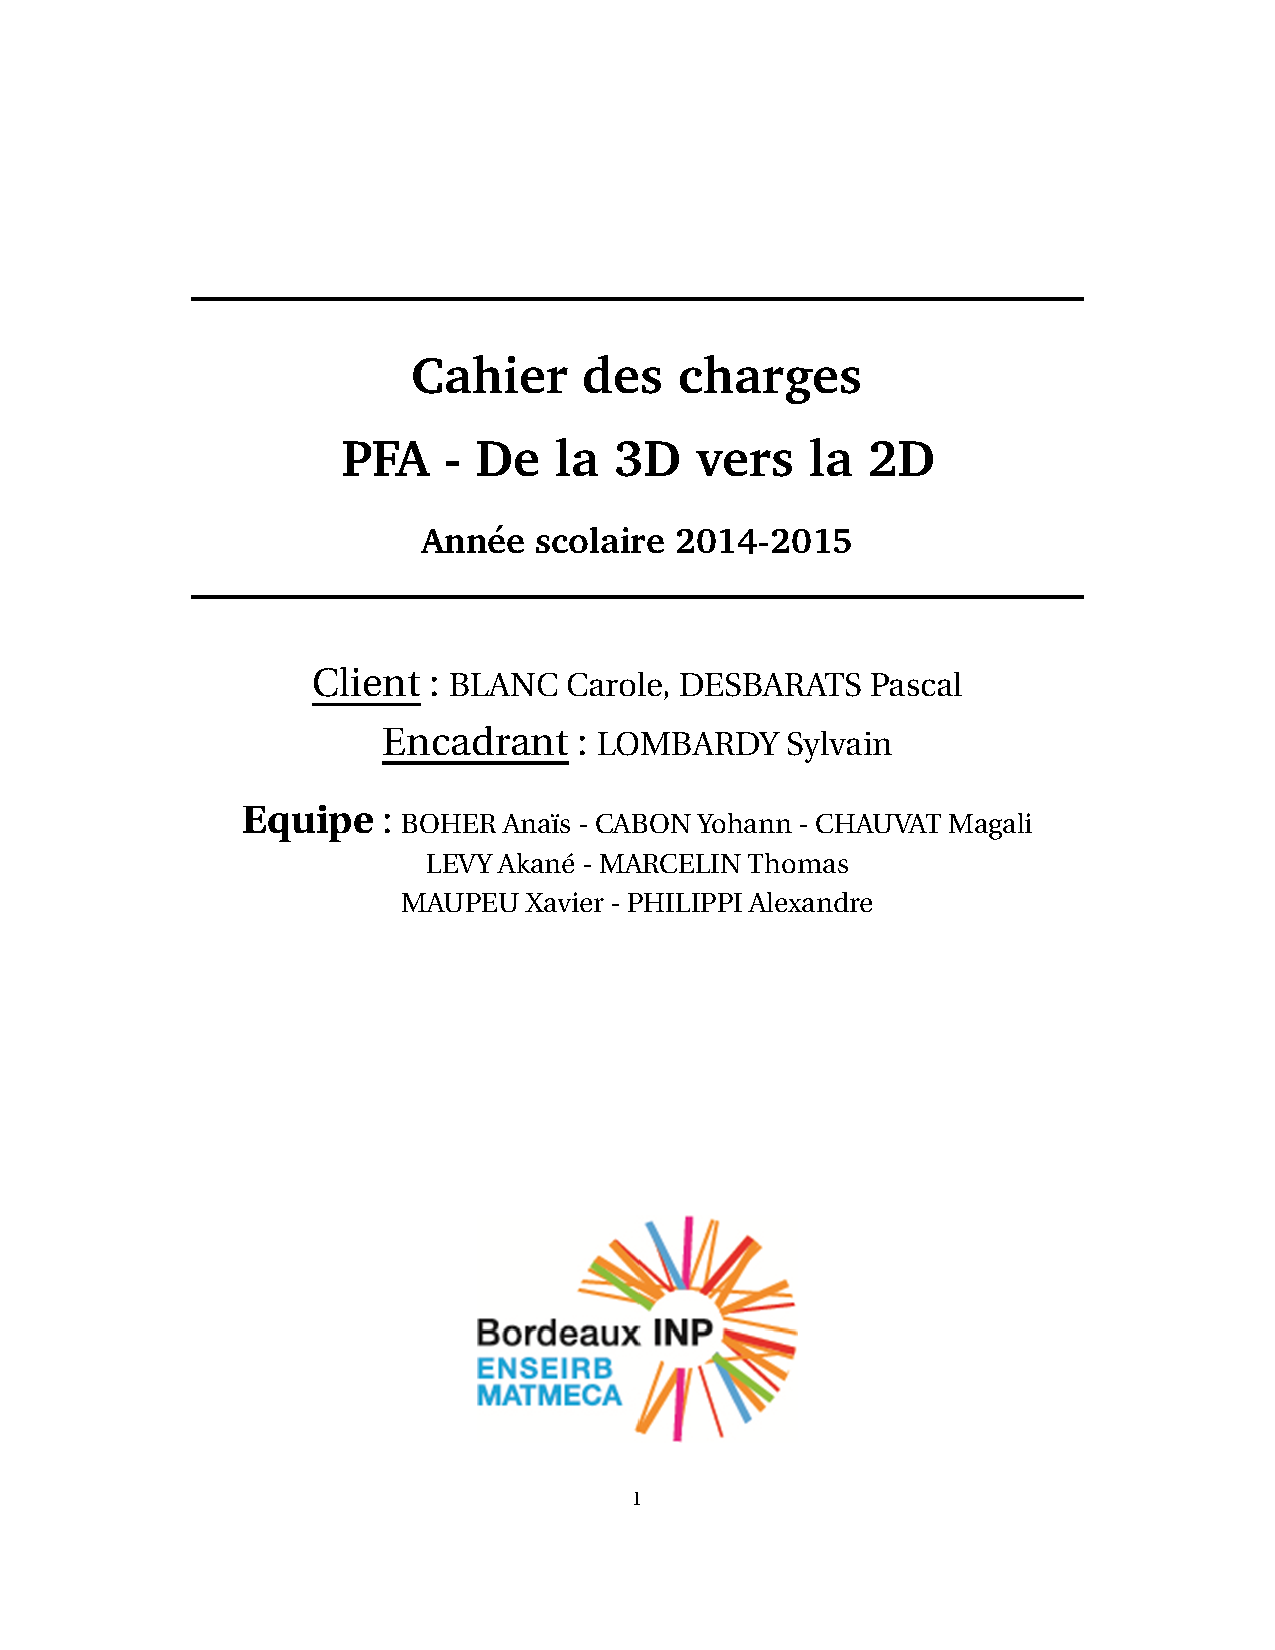
\includepdf[pages=1-29]{cdc.pdf}  
  \newpage
  

  


\end{changemargin}

%%% End document
\end{document}
